\documentclass[10pt, a4paper, oneside]{ctexart}
\usepackage{amsmath, amsthm, amssymb, bm, graphicx, hyperref, mathrsfs}
\usepackage{mdframed}
\usepackage{float}
\usepackage{geometry}
\usepackage{listings}
\usepackage{xcolor}
\usepackage{fancyhdr,url}
\geometry{left=2cm,right=2cm,top=2cm,bottom=2cm}
\hypersetup{
colorlinks=true,
linkcolor=black
}
\lstset{
  language=R,
  basicstyle=\ttfamily,
  keywordstyle=\color{blue},
  commentstyle=\color{green!60!black},
  stringstyle=\color{orange},
  numbers=left,
  numberstyle=\tiny\color{gray},
  stepnumber=1,
  numbersep=5pt,
  backgroundcolor=\color{gray!5},
  frame=single,
  rulecolor=\color{black!30},
  showspaces=false,
  showstringspaces=false,
  showtabs=false,
  tabsize=2,
  captionpos=b,
  breaklines=true,
  breakatwhitespace=true,
}
\fancypagestyle{fancy-license-info}{%
  \fancyhf{}
  \fancyhead[L]{\footnotesize{\leftmark }} 
  \fancyfoot[L]{%
    {\href{http://creativecommons.org/licenses/by-nc-sa/4.0/}{\includegraphics[scale=0.5]{license.eps}}}\hspace{0.1em}%
    \begin{minipage}[b][4ex][t]{30em}
        \footnotesize{本文采用 CC-BY-4.0 授权协议,答案发布于:\\
        \url{https://github.com/yyb100001/Solutions-of-Introduction-to-Probability}\\}
    \end{minipage}
  }
  \fancyfoot[R]{\footnotesize{第 \thepage 页}}
  \renewcommand{\footrulewidth}{0.4pt}
}
\pagestyle{fancy-license-info}
\title{\vspace*{-3cm}\textbf{何书元《概率引论》答案}}
\author{闫一博}
\date{2024年}
\linespread{1.1}
\newenvironment{solution}{\begin{proof}[\bf Solution]}{\end{proof}}
\newenvironment{myproof}{\begin{proof}[\bf Proof]}{\end{proof}}
\mdtheorem[linecolor=black,linewidth=1pt,   frametitlerule=true, nobreak=true]{remark}{remark}

\begin{document}
\maketitle
\tableofcontents 
\newpage 
\section{概率空间}
1.1 验证事件的运算公式:
\[
A\cup B=A+\overline{A}B,\quad A=AB+A\overline{B}
\]
\[\overline {\bigcup\limits_{1 \leqslant j \leqslant n} {{A_j}} }  = \bigcap\limits_{1 \leqslant j \leqslant n} {{{\overline A }_j}},\quad  \overline {\bigcap\limits_{1 \leqslant j \leqslant n} {{A_j}} }  = \bigcup\limits_{1 \leqslant j \leqslant n} {{{\overline A }_j}} \]
\[\overline {\bigcup\limits_{j \geqslant 1} {{A_j}} }  = \bigcap\limits_{j \geqslant 1} {{{\overline A }_j}},\quad  \overline {\bigcap\limits_{j \geqslant 1} {{A_j}} }  = \bigcup\limits_{j \geqslant 1} {{{\overline A }_j}} \]
\begin{myproof}
\[A + \overline A B = A \cup \overline A B = A \cup (\overline A  \cap B) = (A \cup \overline A ) \cap (A \cup B) = A \cup B\]
\[AB + A\bar B = (A \cap B) \cup (A \cap \bar B) = A \cap (B \cup \bar B) = A\]
\[\forall x\quad x \in \overline {\bigcup\limits_{1 \leqslant j \leqslant n} {{A_j}} }  \Leftrightarrow x \notin \bigcup\limits_{1 \leqslant j \leqslant n} {{A_j}}  \Leftrightarrow x \notin {A_j},1 \leqslant j \leqslant n \Leftrightarrow x \in {\overline A _j},1 \leqslant j \leqslant n \Leftrightarrow x \in \bigcap\limits_{1 \leqslant j \leqslant n} {{{\overline A }_j}} \]
\[\forall x\quad x \in \overline {\bigcap\limits_{1 \leqslant j \leqslant n} {{A_j}} }  \Leftrightarrow x \notin \bigcap\limits_{1 \leqslant j \leqslant n} {{A_j}}  \Leftrightarrow \exists {j_1},1 \leqslant {j_1} \leqslant n,x \notin {A_{{j_1}}} \Leftrightarrow x \in {\overline A _{{j_1}}},1 \leqslant {j_1} \leqslant n \Leftrightarrow x \in \bigcup\limits_{1 \leqslant j \leqslant n} {{{\overline A }_j}} \]
\[\forall x\quad x \in \overline {\bigcup\limits_{j \geqslant 1} {{A_j}} }  \Leftrightarrow x \notin \bigcup\limits_{j \geqslant 1} {{A_j}}  \Leftrightarrow x \notin {A_j},j \geqslant 1 \Leftrightarrow x \in \overline {{A}}_j ,j \geqslant 1 \Leftrightarrow x \in \bigcap\limits_{j \geqslant 1} {\overline {A}_j } \]
\[\forall x\quad x \in \overline {\bigcap\limits_{j \geqslant 1} {{A_j}} }  \Leftrightarrow x \notin \bigcap\limits_{j \geqslant 1} {{A_j}}  \Leftrightarrow \exists {j_1},{j_1} \geqslant 1,x \notin {A_{{j_1}}} \Leftrightarrow x \in {\overline A _{{j_1}}},{j_1} \geqslant 1 \Leftrightarrow x \in \bigcup\limits_{j \geqslant 1} {{{\overline A }_j}} \]
\end{myproof}
\begin{remark}
1.1中的后四条均是De Morgan律的推广,无非是有限和可列的区别.
\end{remark}

1.2 用集合的运算表达以下事件

(a)$A$发生、$B$和$C$不发生;(b)$A$不发生、$B$和$C$发生;(c)$A,B,C$都不发生;(d)仅有$A,B,C$之一发生;(e)至少$A,B,C$之一发生.
\begin{solution}
(a)$A\overline{B}\:{\overline{C}}$;(b)$\overline{A}BC$;(c)$\overline{A}\:\overline{B}\:\overline{C}$;(d)$A\overline{B}\:\overline{C}+\overline{A}B\overline{C}+\overline{A}\:\overline{B}C$;(e)$A\cup B\cup C$.
\end{solution}
\begin{remark}
1.2中需要注意区分$\overline{BC}$和$\overline{B}\:\overline{C}$,前者实际是$\overline{B}\cup \overline{C}$(De Morgan律).另外需要注意(e)的描述,常用的方式为$\Omega-\overline{A}\:\overline{B}\:\overline{C}$($\Omega$为三个事件构成的全空间)
\end{remark}

1.3 袋中有大小和质量相同的红、黄、蓝、白球各一个,从中有放回地任取三次,每次一个,并记录下颜色.

(a)写出试验的样本空间;

(b)求取到的三个球颜色互不相同的概率.
\begin{solution}
(a)
\[\Omega  = \{ \omega :\omega  = ({a_1},{a_2},{a_3}),{a_i} \in \{\text{红、黄、蓝、白} \} ,i = 1,2,3\} \]

(b)记取到三个球颜色互不相同为事件$A$,则
\[P(A) = \frac{{C_4^3}\cdot 3!}{{{4^3}}} = \frac{{24}}{{64}} = \frac{3}{8}\]
\end{solution}

1.4 设$\{A_j:j=1,2,\cdots\}$是事件列,求互不相容的$\{B_j:j=1,2,\cdots\}$使得对于$n\geqslant 1$,$\bigcup\limits_{j = 1}^n {{A_j}}  = \bigcup\limits_{j = 1}^n {{B_j}} $和$\bigcup\limits_{j = 1}^\infty  {{A_j}}  = \bigcup\limits_{j = 1}^\infty  {{B_j}} $成立.
\begin{solution}
取$B_1=A_1$,$B_2=A_2-A_1$,以此类推取$B_j=A_j-\bigcup\limits_{i = 1}^{j-1} {{A_i}}(j=2,3,\cdots)$
\end{solution}
\begin{remark}
1.4中的构造非常重要,借助该构造我们可以将任意一列事件转化为一列互斥事件.(类似高代中线性空间的直和分解)
\end{remark}


1.5 $100$件产品中有$3$件次品.

(a)从中任取$2$件,求至少得一件次品的概率;

(b)从中任取$10$件,再从这$10$件中任取$2$件,求至少得一件次品的概率.

\begin{solution}
(a)记任取$2$件且无次品为事件$A$,则
\[P(A) = \frac{{C_{97}^2}}{{C_{100}^2}} \]
记任取$2$件至少有一件次品为事件$B$,则
\[
P(B)=1-P(A)=\frac{147}{2475}
\]
(b)可视作从$100$件产品中取出$10$件不拿出,再从$10$件产品中抽$2$件,故概率与(a)相同.
\end{solution}
\begin{remark}
1.5(b)从逻辑上是很好想通的,因为虽然从$100$件中任取了$10$件,但这$10$件的次品情况仍是未知的,不会改变至少得一件次品的概率,如果从数学上推导则有以下过程:记任取$10$件,再从这$10$件中任取$2$件,无次品为事件$C$,则
\[P(C) = \frac{{C_{97}^{10}C_{10}^2 + C_{97}^9C_3^1C_9^2 + C_{97}^8C_3^2C_8^2 + C_{97}^7C_3^3C_7^2}}{{C_{100}^{10} \cdot C_{10}^2}}\]
\[P(C) = \frac{{97!}}{{100!}} \cdot \left( {\frac{{90!8!}}{{87!8!}} + 3 \cdot \frac{{90!8!}}{{88!7!}} + 3 \cdot \frac{{90!8!}}{{89!6!}} + \frac{{90!8!}}{{90!5!}}} \right) = \frac{{97!}}{{100!}} \cdot \frac{{98!}}{{95!}} \cdot \frac{{C_3^0C_{95}^8 + C_3^1C_{95}^7 + C_3^2C_{95}^6 + C_3^3C_{95}^5}}{{C_{98}^8}}\]
由于
\[\frac{{C_3^0C_{95}^8 + C_3^1C_{95}^7 + C_3^2C_{95}^6 + C_3^3C_{95}^5}}{{C_{98}^8}} = 1\]
故
\[P(C) = \frac{{97!}}{{100!}} \cdot \frac{{98!}}{{95!}} = \frac{{C_{97}^2}}{{C_{100}^2}}=P(A)\]
\end{remark}

1.7 钥匙串上的$5$把钥匙中只有$1$把可以开房门,现在无放回地试开房门.计算

(a)第三次打开房门的概率;

(b)三次内打开房门的概率;

(c)如果$5$把钥匙中有$2$把可以打开房门,求三次内打开房门的概率.

\begin{solution}
记第$i$次打开房门为事件$A_i$,则

(a)记第三次打开房门为事件$B$
\[P(B)=P({\overline A _1}{\overline A _2}{A_3}) = \frac{4}{5} \times \frac{3}{4} \times \frac{1}{3} = \frac{1}{5}\]

(b)记三次内打开房门为事件$C$
\[P(C) = 1 - P({\overline A _1}{\overline A _2}{\overline A _3}) = 1 - \frac{4}{5} \times \frac{3}{4} \times \frac{2}{3} = \frac{3}{5}\]

(c)若有两把钥匙可开门,记三次内打开房门为事件$D$,则
\[P(D) = 1 - P({\overline A _1}{\overline A _2}{\overline A _3}) = 1 - \frac{3}{5} \times \frac{2}{4} \times \frac{1}{3} = \frac{9}{{10}}\]
\end{solution}
\begin{remark}
1.7题是非常简单的,关键在于用事件(集合语言)来描述.
\end{remark}

1.8 设每个人的生日随机落在$365$天中的任一天,求$n$个人的生日互不相同的概率和至少有两个人生日相同的概率.
\begin{solution}
记$n$个人生日互不相同为事件$A$,至少有两个人生日相同为事件$B$,则
\[P(A) = \frac{{C_{365}^n}\cdot n!}{{{{365}^n}}},P(B) = 1 - P(A)\]
\end{solution}


1.9 在$6$副相同的手套中任取四只,计算恰得到一副的概率
\begin{solution}
记在$6$副相同的手套中任取四只,恰得到一副为事件$A$,则
\[P(A) = \frac{{C_6^1C_5^3C_2^1C_2^1}}{{C_{12}^4}} = \frac{{240}}{{495}} = \frac{{16}}{{33}}\]
\end{solution}
\begin{remark}
1.9题有很多种做法,我们这里的思路是先从六副中取一副,剩下的五副中取两副,每副各取一只.
\end{remark}

1.10 从标有$1$至$n$的$n$个球中任取$m$个,记下号码后放回.再从这$n$个球中任取$k$个,记下号码.求两组号码中恰有$c$个号码相同的概率,
\begin{solution}
记两组号码中恰有$c$个号码相同为事件$A$,则
\[P(A) = \frac{{C_m^cC_{n - m}^{k - c}}}{{C_n^k}}\]
\end{solution}
\begin{remark}
1.10题的思路为,将第二次取出的$k$个球分为两类,第一类与$m$个球有相同的号码,第二类与$m$个球的号码不同.
\end{remark}

1.11 在区间$[0,1]$中随机地取两点,求它们的平方和小于$1$的概率.
\begin{solution}
在区间$[0,1]$随机地取两点相互独立,因此可视作在$[0,1]\times [0,1]$中取$(x,y)$,满足$x^2+y^2<1$,也即以原点为圆心$1$为半径的圆,记任取两点平方和小于$1$为事件$A$,则
\[
P(A)=\frac{\pi}{4}
\]
\end{solution}
\begin{remark}
1.11是典型的几何概型,关键在于求面积.
\end{remark}

1.12 二人相约在$5:00-6:00$点之间见面,如果两人在$5:00-6:00$之间独立地随机到达,求一人至少等另一人半小时的概率.
\begin{solution}
记第一人到达的时间为$x$,第二人到达的时间为$y$,即求$P(|x-y|>0.5h)$,记一人至少等另一人半小时为事件$A$,则
\[P(A) = \frac{{2 \times 0.5 \times (0.5 \times 0.5)}}{1\times 1} = \frac{1}{4}\]
\end{solution}

1.13 直径为$1$的硬币随机地落在打有方格的平面上,问方格的边长为多长才能使硬币和网格不相交的概率的概率小于$0.01$.
\begin{solution}
考虑硬币圆心的落点,硬币不与网格相交等价于硬币圆心距离网格边的距离小于半径.设网格边长为$a$,记硬币与网格不相交为事件$A$,则
\[P(A) = \frac{{{{(a - 1)}^2}}}{{{a^2}}} < 0.01\]
$a\leqslant 1$时硬币必与方格相交,故只需考虑$a>1$时的解,由上式可反解$a<\frac{10}{9}$.
\end{solution}
\begin{remark}
 1.13题还可以考虑硬币的外接正方形求解,无论是考虑外接正方形的顶点或是考虑硬币的圆心,画出图像问题就非常直观了.   
\end{remark}

1.14 在同一个小时内有两辆汽车独立到达同一个加油站加油,车$A$加油需要$5$min,车$B$需要$8$min.如果每辆车在这一个小时内等可能的到达,计算这两辆车在加油站不能相遇的概率.
\begin{solution}
记$A$车到达时间为$x$,$B$车到达时间为$y$,即求$P(x-y>5)+P(y-x>8)$,记两辆车在加油站不能相遇为事件$C$,则
\[P(C) = \frac{{0.5 \times ({{55}^2} + {{52}^2})}}{{{{60}^2}}} = \frac{{5729}}{{7200}}\]
\end{solution}
\begin{remark}
1.12和1.14是典型的会面问题,这类问题通常画出图就可以解决.
\end{remark}

1.15 在$[0,1]$中任取三点$X,Y,Z$,求$X^2+Y^2+Z^2\leqslant 1$的概率和$X^2+Y^2+Z^2=1$的概率.
\begin{solution}
  在区间$[0,1]$随机地取三点相互独立,因此可视作在$[0,1]\times [0,1]\times [0,1]$中取$(X,Y,Z)$,满足$X^2+Y^2+Z^2\leqslant 1$和$X^2+Y^2+Z^2=1$,也即以原点为球心$1$为半径的球体和球面,则
\[
P(X^2+Y^2+Z^2\leqslant 1)=\frac{4\pi}{3}\times\frac{1}{8}=\frac{\pi}{6}
\]
根据几何概型的特点,区域边界的测度为零,故
\[
P(X^2+Y^2+Z^2=1)=0
\]  
\end{solution}
\begin{remark}
1.15不过是1.11的推广,这类问题还可以推广至$n$维,本质就是求$n$维球的体积,需要注意的是边界的测度问零.
\end{remark}

例4.3 用$\Omega=\{j:j=1,2,\cdots\}$表示全体正整数,用$B_n=\{j:j=1,2,\cdots,n\}$表示前$n$个正整数.对于$\Omega$的子集$C$,如果极限
\[\mathop {\lim }\limits_{n \to \infty } \frac{{\# (C \cap {B_n})}}{n}\]
存在,则定义
\[P(C) = \mathop {\lim }\limits_{n \to \infty } \frac{{\# (C \cap {B_n})}}{n}\]
现在用$A$表示$\Omega$中能被$m$整除的全体整数,则容易验证$A=\{km:k=1,2,\cdots\}$,并且
\[P(A) = \frac{1}{m},P(\overline A ) = 1 - \frac{1}{m}\]
可以看出$\mathscr{F}=\{\varnothing,A,\overline{A},\Omega\}$是$\sigma$域,$P$是$\mathscr{F}$上的概率,$(\Omega,\mathscr{F},P)$是概率空间.

\newpage
1.16 在例$4.3$中,引入$A_m=\{km:k=1,2,\cdots\}$.计算$P(A_3A_4\overline{A}_5)$.
\begin{solution}
$A_3A_4\overline{A}_5$的含义是能被$12$整除但不能被$60$整除的全体整数,故
\[P({A_3}{A_4}{{\bar A}_5}) = P({A_{12}}) - P({A_{60}}) = \frac{1}{{12}} - \frac{1}{{60}} = \frac{1}{{15}}\]
\end{solution}

1.17 验证概率的次可加性:
\[P(\bigcup\limits_{j = 1}^\infty  {{A_j}) \leqslant } \sum\limits_{j = 1}^\infty  {P({A_j})} \]
\begin{solution}
取$A_0=\varnothing$,${B_j} = {A_j} - \bigcup\limits_{i = 0}^{j - 1} {{A_i}} $,$B_j$互不相容,由于$B_j\subset A_j$,故$ \bigcup\limits_{j = 1}^\infty  {{B_j}}  \subset \bigcup\limits_{j = 1}^\infty  {{A_j}} $.下面验证$ \bigcup\limits_{j = 1}^\infty  {{A_j}}  \subset \bigcup\limits_{j = 1}^\infty  {{B_j}} $,任取$x\in \bigcup\limits_{j = 1}^\infty  {{A_j}}$,存在$i\geqslant 1$(取首个包含$x$的$A_j$对应的下标为$i$),使得$x\in A_i$,但$x\notin A_0,A_1,\cdots,A_{i-1}$(若$i=1$,则$x\notin A_0$),故$x\in B_i$,于是有$ \bigcup\limits_{j = 1}^\infty  {{A_j}}  \subset \bigcup\limits_{j = 1}^\infty  {{B_j}} $,这表明
\[\bigcup\limits_{j = 1}^\infty  {{A_j}}  = \bigcup\limits_{j = 1}^\infty  {{B_j}}\] 根据可列可加性和单调性
\[
P(\bigcup\limits_{j = 1}^\infty  {{A_j}} ) = P(\bigcup\limits_{j = 1}^\infty  {{B_j})}  = \sum\limits_{j = 1}^\infty  {P({B_j})}  \leqslant \sum\limits_{j = 1}^\infty  {P({A_j})} 
\]
\end{solution}
\begin{remark}
1.17题用到了1.4中的构造,在1.4中我们未验证$\bigcup\limits_{j = 1}^\infty  {{A_j}}  = \bigcup\limits_{j = 1}^\infty  {{B_j}}$,证明的关键在于可列性,由于集合可列故可以找到最小的$i$使得$x\in A_i$但是不属于$A_j$,$\forall j<i$.
\end{remark}


1.18 如果事件$A_1,A_2,\cdots$发生的概率都是$1$,证明:
\[P(\bigcap\limits_{j = 1}^\infty  {{A_j}} ) = 1\quad P(\bigcap\limits_{j = 1}^n {{A_j}} ) = 1\]
\begin{solution}
应用De Morgan定律
\[\bigcap\limits_{j = 1}^\infty  {{A_j}}  = \overline {\bigcup\limits_{j = 1}^\infty  {\overline {{A_j}} } } \]
故
\[P(\bigcap\limits_{j = 1}^\infty  {{A_j}} ) = P(\overline {\bigcup\limits_{j = 1}^\infty  {\overline {{A_j}} } } ) = 1 - P(\bigcup\limits_{j = 1}^\infty  {\overline {{A_j}} } )\]
根据概率的次可加性
\[0 \leqslant P(\bigcup\limits_{j = 1}^\infty  {\overline {{A_j}} } ) \leqslant \sum\limits_{j = 1}^\infty  {P(\overline {{A_j}} )}  = \sum\limits_{j = 1}^\infty  {(1 - P({A_j}))}  = \sum\limits_{j = 1}^\infty  0=0 \]
综上可得
\[P(\bigcap\limits_{j = 1}^\infty  {{A_j}} ) = 1 - P(\bigcup\limits_{j = 1}^\infty  {\overline {{A_j}} } ) = 1\]
同理可证,$P(\bigcap\limits_{j = 1}^n {{A_j}} ) = 1$
\end{solution}

1.19 对于事件$A,B$,验证
\[
P(AB)+P(\overline{A}B)+P(A\overline{B})+P(\overline{A}\:\overline{B})=1
\]
\begin{solution}
$AB,\overline{A}B,A\overline{B},\overline{A}\:\overline{B}$互不相容,由可列(有限)可加性
\[P(AB) + P(\bar AB) + P(A\bar B) + P(\bar A\:\bar B) = P(AB \cup \bar AB \cup A\bar B \cup \bar A\:\bar B) = P(B \cup \bar B) = 1\]
\end{solution}

1.20 设$A_1\subset A_2\subset \cdots$,$P(A_j)=(1-1/j)^j$.计算$P(\bigcup\limits_{j = 1}^\infty  {{A_j}} )$.
\begin{solution}
$\{A_j\}$是单调增序列,故
\[
P(\bigcup\limits_{j = 1}^\infty  {{A_j}} ) = \mathop {\lim }\limits_{n \to \infty } P({A_n}) = \mathop {\lim }\limits_{n \to \infty } {(1 - \frac{1}{j})^j} = \frac{1}{e}
\]
\end{solution}
\begin{remark}
1.20不过是概率的连续性的简单应用,概率作为测度其最重要的三个性质就是:单调性、次可加性、连续性.
\end{remark}

1.21 重复地投掷一枚硬币$100$次,用$1,0$分别表示得到正、反面.依次记录正反面出现的情况.

以下是用R语言模拟的结果及代码
\begin{figure}[h]
    \centering
    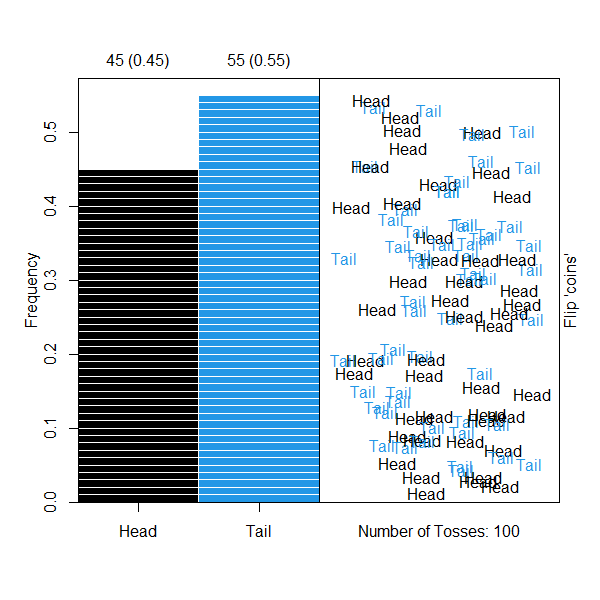
\includegraphics[width=0.5\linewidth]{1.21.png}
\end{figure}
\begin{lstlisting}
library(animation)
ani.options(interval = 0.2, nmax = 100)
flip.coin(faces = c("Head", "Tail"),type = "n",prob = c(0.5, 0.5),col = c(1, 4))
\end{lstlisting}

\newpage
\section{加法和乘法公式}
2.1 甲毕业时在单位A求职成功的概率为$0.4$,在单位B求职成功的概率为$0.6$,在这两家都求职成功的概率为$0.24$.如果甲在这两个单位都求职,计算他至少被一家录用的概率.
\begin{solution}
记甲被单位$A$录取为事件$A$,被单位$B$录取为事件$B$,根据加法公式,
\[P(A \cup B) = P(A) + P(B) - P(AB) = 0.4 + 0.6 - 0.24 = 0.76\]
\end{solution}

2.2 $9$个学生随机走进$3$个自习室.

(a)求至少有一个自习室无学生的概率;

(b)求每个自习室至少有一个学生的概率.
\begin{solution}
每个学生走进自习室相互独立

(a)记第$i$个自习室无学生为事件$A_i$,根据Jordan公式
\[P({A_1} \cup {A_2} \cup {A_3}) = \sum\limits_{i = 1}^3 {P({A_i})}  - \sum\limits_{1 \leqslant i < j \leqslant 3}^3 {P({A_i}{A_j})}  + P(\bigcap\limits_{i = 1}^3 {{A_i}} )\]
其中
\[P({A_i}) = \frac{{{2^9}}}{{{3^9}}},P({A_i}{A_j}) = \frac{{{1^9}}}{{{3^9}}},P(\bigcap\limits_{i = 1}^3 {{A_i}} ) = 0\]
代入可得
\[P({A_1} \cup {A_2} \cup {A_3}) = 3 \cdot \frac{{{2^9}}}{{{3^9}}} - 3 \cdot \frac{{{1^9}}}{{{3^9}}} + 0 = \frac{{511}}{{6561}}\]

(b)记每个自习室至少有一个学生为事件$B$,则
\[P(B) = 1 - P({A_1} \cup {A_2} \cup {A_3}) = \frac{{6050}}{{6561}}\]
\end{solution}
\begin{remark}
2.2是对Jordan公式的简单应用,具体的讲是一种特殊情形,即概率与选择元素的次序无关,而只与选择元素的个数有关.下面的2.3,2.4都是同一类问题.
\end{remark}

2.3 $6$个人将各自的帽子混在一起后每人任取一项,求没有人取得自己帽子的概率.
\begin{solution}
记第$i$个人没有取到自己的帽子为事件$A_i$,则$\overline{A}_i$表示第$i$个人取到了自己的帽子,根据De Morgan定律
\[P(\bigcap\limits_{i = 1}^6 {{A_i}} ) = 1 - P(\bigcup\limits_{i = 1}^6 {{{\overline A }_i}} )\]
根据Jordan公式
\[P(\bigcup\limits_{i = 1}^6 {{{\overline A }_i}} ) = \sum\limits_{n = 1}^6 {{{( - 1)}^{n - 1}}C_6^n\frac{{(6 - n)!}}{{6!}}}  = \sum\limits_{n = 1}^6 {{{( - 1)}^{n - 1}}\frac{1}{{n!}}} \]
故
\[P(\bigcap\limits_{i = 1}^6 {{A_i}} ) = 1 - \sum\limits_{n = 1}^6 {{{( - 1)}^{n - 1}}\frac{1}{{n!}}}  = \sum\limits_{n = 0}^6 {{{( - 1)}^n}\frac{1}{{n!}}} \]
\end{solution}
\begin{remark}
2.3得到的结果是有趣的,当人数趋于无穷时,根据$e^x$的Taylor展开式可得
\[P(\bigcap\limits_{i = 1}^\infty  {{A_i}} ) = \sum\limits_{n = 0}^\infty  {{{( - 1)}^n}\frac{1}{{n!}}}  = \frac{1}{e}\]
\end{remark}

\newpage
2.4 开学时老师声明本学期要点名$m$个人,每次都是又放回的随机点名.当全班有$n$个学生,计算

(a)你在本学期不被点到的概率;

(b)当$n\leqslant m$,至少有一个学生在本学期不被点到的概率.
\begin{solution}
(a)记一名同学一学期不被点到为事件$A$,由于每次点名独立,故
\[P(A) = {\left( {1 - \frac{1}{n}} \right)^m}\]

(b)记第$i$个学生未被点到为事件$A_i$,则至少有一个学生未被点到的概率为$P(\bigcup\limits_{i = 1}^n {{A_i}})$,由于\[P({A_i}) = \frac{{{{(n - 1)}^m}}}{{{n^m}}},P({A_i}{A_j}) = \frac{{{{(n - 2)}^m}}}{{{n^m}}}, \cdots \]根据Jordan公式
\[P(\bigcup\limits_{i = 1}^n {{A_i}} ) = \sum\limits_{k = 1}^n {{{( - 1)}^{k - 1}}} C_n^k\frac{{{{(n - k)}^m}}}{{{n^m}}}\]
\end{solution}
\begin{remark}
2.3和2.4本质上讲是一样的,区别在于2.3无放回(拿走的帽子无法再被拿走),2.4有放回(被点名的同学还可能再被点到).
\end{remark}

2.5 将$n$个不同的信笺随机放入$n$个写好地址的信封,求至少有一封匹配的概率.
\begin{solution}
记第$i$封信封与信笺匹配为事件$A_i$,根据Jordan公式
\[P(\bigcup\limits_{i = 1}^n {{A_i})}  = \sum\limits_{i = 1}^n {P({A_i})}  + {( - 1)^{m - 1}}\sum\limits_{1 \leqslant {i_1} < {i_2} <  \cdots  < {i_m} \leqslant n} {P({A_{{i_1}}}{A_{{i_2}}} \cdots {A_{{i_m}}})}  + {( - 1)^{n - 1}}P(\bigcap\limits_{i = 1}^n {{A_i})} \]
于是有
\[P(\bigcup\limits_{i = 1}^n {{A_i})}  = \sum\limits_{m = 1}^n {{{( - 1)}^{m - 1}}C_n^m\frac{{(n - m)!}}{{n!}}}  = \sum\limits_{m = 1}^n {{{( - 1)}^{m - 1}}\frac{1}{{m!}}} \]
\end{solution}
\begin{remark}
2.5与2.3并无本质区别,不过是进一步推广.
\end{remark}

2.6 $6$个人独立破译同一个密码.当第$j$个人能破译密码的概率为$p_j$,计算密码被破译的概率.
\begin{solution}
记第$j$个人破译成功为事件$A_j$,根据De Morgan定律
\[P(\bigcup\limits_{j = 1}^6 {{A_j}} ) = 1 - P(\bigcap\limits_{j = 1}^6 {{{\overline A }_j}} )\]
由于$6$个人未成功破译密码相互独立,故
\[P(\bigcup\limits_{j = 1}^6 {{A_j}} ) = 1 - \prod\limits_{j = 1}^6 {(1 - {p_j})} \]
\end{solution}

2.7 在旷野迷路后,甲每隔一小时发出一个求救信号,如果每个信号被搜救队发现的概率是$0.1$,要以$0.95$的概率保证搜救队能发现信号,甲至少要发送多少个信号?
\begin{solution}
记甲发出的第$j$个信号被接受为事件$A_j$,根据De Morgan定律
\[P(\bigcup\limits_{j = 1}^n {{A_j}} ) = 1 - P(\bigcap\limits_{j = 1}^n {{{\bar A}_j}} )\]
由于每个信号未被接受相互独立,故
\[P(\bigcup\limits_{j = 1}^n {{A_j}} ) = 1 - \prod\limits_{j = 1}^n {0.9}  = 1 - {0.9^n}\]
由题意知
\[1 - {0.9^n} \geqslant 0.95 \Rightarrow {0.9^n} < 0.05 \Rightarrow n > {\log _{0.9}}(0.05) \Rightarrow n \geqslant 29\]
\end{solution}
\begin{remark}
2.6和2.7是同一类型的问题,求解的关键在于用逆事件描述问题,以2.7为例,第一个信号是否被收到会影响第二个信号是否发出,记第$j$个信号未被接受为事件$B_j$,搜救队未发现信号的概率记作$p_n$,用乘法公式表述则有:
\[
\begin{aligned}
{p_n} &= P({B_1}{B_2} \cdots {B_n})\\
& = P({B_1})P({B_2}|{B_1}) \cdots P({B_n}|{B_1}{B_2} \cdots {B_{n - 1}})\\
& = 0.9\times0.9\times \cdots \times 0.9\\
& = 0.9^n
\end{aligned}
\]
一旦意识到每个信号未被接受是独立的,则上面的过程是多余的.
\end{remark}

2.8 通常认为产品的名称会影响其销量.对一种新产品现在有两种起名方案备选.方案$1$是邀请$4$名相关专家起名,厂家向起名成功者支付$2$万元奖励,对其余$3$名各支付$5$千元的酬金.方案二是悬赏$2$万元在互联网上征名.如果所请的每个专家能独立想出满意名称的概率为$60\%$,互联网上的每个人能独立想出满意名称的概率为$1\%$.

(a)计算方案$1$成功的概率;

(b)如果有$500$个人在网上参与起名,计算方案$2$成功的概率.
\begin{solution}
(a)每个专家是否想出满意名称相互独立,记第$i$个专家想出满意名称为事件$A_i$,根据De Morgan定律
\[P(\bigcup\limits_{i = 1}^4 {{A_i}} ) = 1 - P(\bigcap\limits_{i = 1}^4 {{{\overline A }_i}} ) = 1 - {0.4^4} = 0.9744\]

(b)记互联网上第$j$个人想出满意名称为事件$B_j$,根据De Morgan定律
\[P(\bigcup\limits_{j = 1}^{500} {{B_j}} ) = 1 - P(\bigcap\limits_{j = 1}^{500} {{{\overline B }_j}} ) = 1 - {0.99^{500}} = 0.9934\]
\end{solution}
\begin{remark}
笔者认为2.8题存在一些问题,如果$4$名专家都想出了满意名称,则题目所述的奖励方案不成立.(事实上,本题与奖励方案无关)
\end{remark}

2.9 $12$小时内,每个破译员能够成功破译刚截获的密码的概率(称为破译能力)不小于$0.05$,现在上级派来$5$位破译能力达到$0.2$的专家参加工作,需要再配备多少破译员才能使得密码被破译的概率达到$0.95$.
\begin{solution}
记$12$小时内密码未被破译为事件$A$,记第$i$名专家未破译密码为事件$A_i$,第$j$名破译员未破译密码为事件$B_j$,现求破译员人数使得$P(A)<0.05$,即求$n$使得
\[P(A) = P({A_1} \cdots {A_5}{B_1} \cdots {B_n}) < 0.05\]
由于每人未破译密码相互独立,故
\[P(A) = {(0.8)^5}{(0.95)^n}\]
于是有
\[{(0.8)^5}{(0.95)^n} < 0.05 \Rightarrow n \geqslant 37\]
\end{solution}

2.10 投掷两个筛子$24$次,至少掷出一对$6$的概率小于二分之一,证明这一结论
\begin{myproof}
记投掷$24$次两个筛子没有出现一对$6$为事件$A$,则
\[P(A) = {\left( {\frac{{35}}{{36}}} \right)^{24}} > \frac{1}{2}\]
这表明掷$24$次两个筛子至少掷出一对$6$的概率小于二分之一.
\end{myproof}
\begin{remark}
2.10中${\left( {\frac{{35}}{{36}}} \right)^{24}} > \frac{1}{2}$用计算器容易验证,如果不借助计算器而对${\left( {\frac{{35}}{{36}}} \right)^{24}}$进行估计,则可以采用以下方式:
\[24\ln (1 - \frac{1}{{36}}) + \ln 2 = \ln 2 - 24(\frac{1}{{36}} + \frac{1}{2}\frac{1}{{{{36}^2}}} +  \cdots ) = \ln 2 - 24(\frac{1}{{36}} + \frac{1}{{2{{(1 - \xi )}^2}}}\frac{1}{{{{36}^2}}}),\xi  \in (0,\frac{1}{{36}})\]
于是有
\[24\ln (1 - \frac{1}{{36}}) + \ln 2 > \ln 2 - \frac{2}{3} - \frac{{12}}{{{{(35)}^2}}} > 0 \Rightarrow {\left( {\frac{{35}}{{36}}} \right)^{24}} > \frac{1}{2}\]
\end{remark}

2.11 无论哪门课先考,甲的微积分和线性代数得优的概率分别是$a$和$b$,微积分先考并得优的条件下,线性代数得优的概率是$c$.当微积分先考时,计算

(a)甲的这两门都得优的概率;(b)微积分没得优的条件下,线性代数得优的概率;(c)线性代数得优的概率;(d)至少一门得优的概率;(e)至少一门不得优的概率.
\begin{solution}
记甲微积分得优为事件$A$,线性代数得优为事件$B$

(a)
\[P(AB) = P(A)P(B|A) = ac\]

(b)\[P(B|\bar A) = \frac{{P(\bar AB)}}{{P(\bar A)}} = \frac{{P(B) - P(AB)}}{{P(\bar A)}} = \frac{{b - ac}}{{1 - a}}\]

(c)
\[P(B) = P(A)P(B|A) + P(\bar A)P(B|\bar A) = b\]

(d)
\[P(A \cup B) = P(A) + P(B) - P(AB) = a + b - ac\]

(e)
\[P(\overline A  \cup \overline B ) = 1 - P(AB) = 1 - ac\]
\end{solution}

2.12 一架相机第一次落地摔坏的概率是$0.5$.若第一次没摔坏,第二次落地摔坏的概率是$0.7$.若第二次没摔坏,第三次落地摔坏的概率为$0.9$.求该相机落地三次没有摔坏的概率.
\begin{solution}
记第$i$次落地没有摔坏为事件$A_i$,则
\[P({A_1}{A_2}{A_3}) = P({A_1})P({A_2}|{A_1})P({A_3}|{A_1}{A_2}) = 0.5 \times 0.3 \times 0.1 = 0.015\]
\end{solution}
\begin{remark}
注意2.12题目中给出的概率是条件概率.
\end{remark}

2.13 投掷$2$个均匀的骰子,已知至少有一个骰子的点数是$3$,

(a)计算这两个骰子的点数之和为$7$的概率;(b)你应当猜这两个骰子的点数之和是$7$还是$6$.
\begin{solution}
记第一个骰子掷出点数$i$为事件$A_i$,第二个骰子掷出点数$i$为事件$B_i$,则$A_3\cup B_3$表示至少有一个骰子的点数是$3$

(a)记两个骰子点数之和为$7$为事件$A$,则
\[P(A|{A_3} \cup {B_3}) = \frac{{P({A_4}{B_3} \cup {A_3}{B_4})}}{{P({A_3} \cup {B_3})}} = \frac{2}{{11}}\]

(b)记两个骰子点数之和为$6$为事件$B$,则
\[P(B|{A_3} \cup {B_3}) = \frac{{P({A_3}{B_3})}}{{P({A_3} \cup {B_3})}} = \frac{1}{{11}}\]
应当猜$7$.
\end{solution}
\begin{remark}
2.13除上述方法外还可以考虑古典概型计算有利场合数的方法,已知至少有一个骰子的点数是$3$将改变样本空间.
\end{remark}

2.14 某官员第$1$次受贿没被查处的概率是$q_1=98/100=0.98$.第$1$次没被查处后,第$2$次受贿没被查处的概率是$q_2=96/98=0.9796,\cdots$.前$j-1$次没被查处后,第$j$次受贿没被查处的概率是$q_j=(100-2j)/(100-2(j-1)),\cdots$.

(a)计算他受贿$n$次还不被查处的概率;(b)假设$q_1=q_2=\cdots=0.98$,计算他受贿$n$次还不被查处的概率.
\begin{solution}
记官员第$j$次受贿没被查处为事件$A_j$

(a)
\[P({A_1}{A_2} \cdots {A_n}) = P({A_1})P({A_2}|{A_1}) \cdots P({A_n}|{A_1}{A_2} \cdots {A_{n - 1}})\]
将题目所给概率代入可得
\[P({A_1}{A_2} \cdots {A_n}) = \frac{{98}}{{100}} \times \frac{{96}}{{98}} \times  \cdots  \times \frac{{100 - 2n}}{{100 - 2(n - 1)}} = 1 - \frac{n}{{50}},n\leqslant 50\]

(b)若$q_1=q_2=\cdots=0.98$,则有
\[P({A_1}{A_2} \cdots {A_n}) = {0.98^n}\]
\end{solution}

2.15 尽管通常都假设男女婴儿的出生率是相同的,但是大量的统计资料表明男婴的出生率一般高于女婴的出生率.现在假设男婴的出生率是$p=0.51$,女婴的出生率是$q=0.49$.如果新同事家有两个年龄不同的小孩,且已知他家至少有一个女孩,计算另一个也是女孩的概率.
\begin{solution}
记第一个孩子是女孩为事件$A$,第二个孩子是女孩为事件$B$,则
\[P(AB|A \cup B) = \frac{{P(AB)}}{{P(A \cup B)}} = \frac{{{{0.49}^2}}}{{1 - {{0.51}^2}}} = 0.3245\]
\end{solution}
\begin{remark}
2.15是仿照2.13的过程,事实上,记至少有一个女孩为事件$A$,两个都是女孩为事件$B$,则
\[P(B|A) = \frac{{P(AB)}}{{P(A)}} = \frac{{{{0.49}^2}}}{{1 - {{0.51}^2}}} = 0.3245\]
\end{remark}

2.16 老板有一个不很负责的秘书.当要秘书通知张经理$5$小时后见面时,秘书马上办理,但是只用某种方式通知一次.设秘书用传真通知的概率是$0.3$,用短信通知的概率是$0.2$,用电子邮件通知的概率为$0.5$,而张经理在$5$小时内能收到传真的概率是$0.8$,能看到短信的概率是$0.9$,能看到电子邮件的概率是$0.4$.

(a)计算张经理收到通知的概率;

(b)如果收到通知的张经理也有$5$\%的概率不能来见老板,计算老板不能按时见到张经理的概率;
\begin{solution}
(a)记张经理收到通知为事件$A$,根据全概率公式
\[P(A) = 0.3 \times 0.8 + 0.2 \times 0.9 + 0.5 \times 0.4 = 0.62\]

(b)记张经理按时来见老板为事件$B$,根据全概率公式
\[P(B) = P(A)P(B|A) + P(\overline A )P(B|\overline A ) = 0.62 \times 0.95 + 0.38 \times 0 = 0.589\]
因此张经理不能按时来见老板的概率为$P(\overline{B})=1-P(B)=0.411$.
\end{solution}
\begin{remark}
记张经理不能按时来见老板为事件$C$,根据全概率公式
\[P(C) = P(A)P(C|A) + P(\bar A)P(C|\bar A) = 0.62 \times 0.05 + 0.38 \times 1 = 0.411\]
\end{remark}

2.17 在调查家庭暴力所占家庭的比例$p$时,为得到实际的$p$同时又不侵犯个人隐私,调查人员将袋中放入比例是$p_0$的红球和比例是$q_0=1-p_0$的白球.被调查者在袋中任取一球窥视后放回,并承诺取得红球就讲真话,取到白球就将假话.被调查者只需在匿名调查表中选“是”或“否”,然后将表放入投票箱.没人能知道被调查者是否讲真话和回答的是什么.

(a)如果声称有家庭暴力的家庭比例是$p_1$,求$p$;

(b)如果袋中装有$30$个红球,$50$个白球,调查了$320$个家庭,其中有$195$个家庭回答了是,估算$p$;
\begin{solution}
(a)记调查家庭回答“是”为事件$A$,抽到红球为事件$B$,则$P(B)=p_0$,$P(\overline{B})=q_0$,$P(A|B)=p$,$P(A|\overline{B})=1-p$,根据全概率公式
\[{p_1} = P(A) = P(B)P(A|B) + P(\overline B )P(A|\overline B ) = {p_0}p + {q_0}(1 - p)\]
于是有
\[p = \frac{{{p_1} - {q_0}}}{{{p_0} + {q_0}}}\]
(b)将数据带入
\[p = \frac{{{p_1} - {q_0}}}{{{p_0} - {q_0}}} = \frac{{\frac{{195}}{{320}} - \frac{5}{8}}}{{\frac{3}{8} - \frac{5}{8}}} = \frac{5}{{80}} = 6.25\% \]
\end{solution}

2.18 一枚深水炸弹击沉、击伤和不能击中一艘潜水艇的概率分别为$1/3,1/2,1/6$.设击伤该潜水艇两次也使该潜水艇沉没,求用$4$枚深水炸弹击沉该潜艇的概率.
\begin{solution}
记$4$枚深水炸弹未击沉该潜艇为事件$A$
\[P(A) = {\left( {\frac{1}{6}} \right)^4} + C_4^1{\left( {\frac{1}{6}} \right)^3}\left( {\frac{1}{2}} \right) = 0.01\]
因此$4$枚深水炸弹击沉该潜艇的概率为$P(\overline{A})=1-P(A)=0.99$.
\end{solution}
\begin{remark}
2.18如果从正面分析则情况繁多,计算较为复杂,若计算逆事件的概率则简洁明了.
\end{remark}

2.19 两人下棋,每局获胜者得一分,累积多于对手两分者获胜.设甲每局获胜的概率是$p$,求甲最终获胜的概率.
\begin{solution}
(i)不考虑平局,记甲赢第一局为事件$A$,甲领先$k$分时最终获胜为事件$B_k$,记$q(k)=P(B_k)$,已知$A$发生时,甲领先一分,$P(B_k|A)=P(B_{k+1})=q(k+1)$,同理可得$P(B_k|\overline{A})=q(k-1)$,由题意$P(A)=p$,记$P(\overline{A})=r$,根据全概率公式
\[q(k) = P({B_k}) = P(A)P({B_k}|A) + P(\overline A )P({B_k}|\overline A ) = pq(k + 1) + rq(k - 1)\]
可得递推关系式
\[q(k) = pq(k + 1) + rq(k - 1)\]
甲最终获胜的概率即$q(0)$,由于$q(2)=1,q(-2)=0$于是有
\[q(0) = pq(1) + rq( - 1) = p\left( {pq(2) + rq(0)} \right) + r\left( {pq(0) + rq( - 2)} \right) = {p^2} + 2prq(0)\]
故
\[q(0) = \frac{{{p^2}}}{{1 - 2pr}} = \frac{{{p^2}}}{{{{(p + r)}^2} - 2pr}} = \frac{{{p^2}}}{{{p^2} + {r^2}}}\]
(ii)考虑平局,记甲赢第一局、平局、输第一局分别为事件$A,B,C$,同(i)分析过程,根据全概率公式
\[q(k) = P({B_k}) = P(A)P({B_k}|A) + P(B)P({B_k}|B) + P(C)P({B_k}|C) = pq(k + 1) + (1 - p - r)q(k) + rq(k - 1)\]
可得递推关系式
\[q(k) = pq(k + 1) + (1 - p - r)q(k) + rq(k - 1) \Rightarrow q(k) = \frac{p}{{p + r}}q(k + 1) + \frac{r}{{p + r}}q(k - 1)\]
于是有
\[q(0) = \frac{p}{{p + r}}q(1) + \frac{r}{{p + r}}q( - 1) = \frac{p}{{p + r}}\left( {\frac{p}{{p + r}}q(2) + \frac{r}{{p + r}}q(0)} \right) + \frac{r}{{p + r}}\left( {\frac{p}{{p + r}}q(0) + \frac{r}{{p + r}}q( - 2)} \right)\]
故
\[\left( {1 - \frac{{2rp}}{{{{(p + r)}^2}}}} \right)q(0) = \frac{{{p^2}}}{{{{(p + r)}^2}}} \Rightarrow q(0) = \frac{{{p^2}}}{{{p^2} + {r^2}}}\]
\end{solution}
\begin{remark}
2.19在不考虑平局时,只有当一方连赢两局游戏才会结束,记游戏结束为事件$A$,甲获胜为事件$B$,则
\[P(B|A) = \frac{{P(AB)}}{{P(A)}} = \frac{{{p^2}}}{{{p^2} + {r^2}}}\]
\end{remark}

2.20 设医生有黑、红两种新药品治疗同一种疾病,疗效未知.如何决定用哪种药是医生所关心的问题.统计学家建议医生将口袋里放入$b$个黑球和$r$个红球后任取一球.取到黑球用黑药,并将球放回.取到红球用红药,并将球放回.如果药物有效就再在袋中假如同一颜色的球一只.用$B_i$表示第$i$次取到黑球,如果两种药都是百分之百的有效.

(a)计算$P(B_1B_2B_3)$;

(b)计算$P(B_2)$,$P(B_3)$;

(c)试用归纳的方法计算$P(B_n)$.
\begin{solution}
(a)由于药百分之百有效,根据乘法公式
\[P({B_1}{B_2}{B_3}) = P({B_1})P({B_2}|{B_1})P({B_3}|{B_1}{B_2}) = \frac{b}{{b + r}} \times \frac{{b + 1}}{{b + r + 1}} \times \frac{{b + 2}}{{b + r + 2}}\]
(b)根据全概率公式
\[P({B_2}) = P({B_1})P({B_2}|{B_1}) + P({\overline B _1})P({B_2}|{\overline B _1}) = \frac{b}{{b + r}} \times \frac{{b + 1}}{{b + r + 1}} + \frac{r}{{b + r}} \times \frac{b}{{b + r + 1}} = \frac{b}{{b + r}}\]
\[P({B_3}) = P({B_1}{B_2})P({B_3}|{B_1}{B_2}) + P({\overline B _1}{B_2})P({B_3}|{\overline B _1}{B_2}) + P({B_1}{\overline B _2})P({B_3}|{B_1}{\overline B _2}) + P({\overline B _1}{\overline B _2})P({B_3}|{\overline B _1}{\overline B _2})\]
于是有
\[P({B_3}) = \frac{{b(b + 1)}}{{(b + r)(b + r + 1)}} \cdot \frac{{b + 2}}{{b + r + 2}} + \frac{{2rb}}{{(b + r)(b + r + 1)}} \cdot \frac{{b + 1}}{{b + r + 2}} + \frac{{r(r + 1)}}{{(b + r)(b + r + 1)}} \cdot \frac{b}{{b + r + 2}}\]
整理得到
\[P({B_3}) = \frac{{b(b + 1)(b + 2) + 2rb(b + 1) + r(r + 1)b}}{{(b + r)(b + r + 1)(b + r + 2)}} = \frac{b}{{b + r}} \cdot \frac{{{b^2} + 3b + 2 + 2rb + 2r + {r^2} + r}}{{{b^2} + rb + 2b + rb + {r^2} + 2r + b + r + 2}} = \frac{b}{{b + r}}\]
(c)对于$n=1$,$P(B_1)=\frac{b}{b+r}$成立,假设对于$n-1$成立$P(B_{n-1})=\frac{b}{b+r}$.已知$B_1$发生后,$B_n$变为$b+1$个黑球和$r$个红球的$B_{n-1}$,根据归纳假设
\[P({B_n}|{B_1}) = \frac{{b + 1}}{{b + r + 1}}\]
同理可得($B_1$不发生则为$b$个黑球和$r+1$个红球情形)
\[P({B_n}|{\overline B _1}) = \frac{b}{{b + r + 1}}\]
根据全概率公式
\[P({B_n}) = P({B_1})P({B_n}|{B_1}) + P({\overline B _1})P({B_n}|{\overline B _1}) = \frac{b}{{b + r}} \times \frac{{b + 1}}{{b + r + 1}} + \frac{r}{{b + r}} \times \frac{b}{{b + r + 1}} = \frac{b}{{b + r}}\]
\end{solution}
\begin{remark}
2.20需注意归纳法的使用,其本质依旧是抽签原理.(药效为百分之百)通常的教材往往只计算$B_2$,笔者用全概率公式计算了$B_3$情形,是对抽签原理的进一步验证,事实上这样做并无任何难度.
\end{remark}

2.21 甲成汽车、火车的概率分部为$0.6,0.4$.汽车和火车正点到达的概率分别是$0.8$和$0.9$.现在甲已经正点到达,求甲乘的是火车的概率.
\begin{solution}
记甲乘火车为事件$A$,甲正点到达为事件$B$,根据全概率公式
\[P(B) = P(A)P(B|A) + P(\overline A )P(B|\overline A ) = 0.4 \times 0.9 + 0.6 \times 0.8 = 0.84\]
再根据Bayes公式,有
\[P(A|B) = \frac{{P(A)P(B|A)}}{{P(B)}} = \frac{{0.4 \times 0.9}}{{0.84}} = \frac{3}{7}\]
\end{solution}


2.22 一台机床工作状态良好时,产品的合格率为$99\%$,机床发生故障时的产品合格率为$50\%$.设每次新开机器时机床处于良好状态的概率为$95\%$.如果新开机器后生产的第一件产品是合格品,判断机器处于良好状态的概率.
\begin{solution}
记机床工作状态良好为事件$A$,新开机器后生产的产品是合格品为事件$B$,根据全概率公式和Bayes公式
\[P(A|B) = \frac{{P(A)P(B|A)}}{{P(B)}} = \frac{{0.95 \times 0.99}}{{0.95 \times 0.99 + 0.05 \times 0.5}} = 0.9741\]
\end{solution}

2.23 一种新方法检测出某种疾病的概率是百分之百,但是把没病的人判定有病的概率达到百分之五.设群体中该病的发病率是万分之一.

(a)甲在身体普查中被判断患病,甲的确患病的概率是多少?

(b)甲再次复查又被判断有病时,甲的确患病的概率是多少?
\begin{solution}
记甲的确患病为事件$A$,被判断患病为事件$B$

(a)根据全概率公式
\[P(B) = P(A)P(B|A) + P(\overline A )P(B|\overline A ) = 0.0001 \times 1 + 0.9999 \times 0.05 = 0.050095\]
根据Beyes公式
\[P(A|B) = \frac{{P(A)P(B|A)}}{{P(B)}} = \frac{{0.0001 \times 1}}{{0.050095}} = 0.00199\]

(b)经过普查后甲患病率变为千分之二,根据全概率公式
\[P(B) = P(A)P(B|A) + P(\overline A )P(B|\overline A ) = 0.002 \times 1 + 0.998 \times 0.05 = 0.0519\]
根据Bayes公式
\[P(A|B) = \frac{{P(A)P(B|A)}}{{P(B)}} = \frac{{0.002 \times 1}}{{0.0519}} = 0.0385\]
\end{solution}
\begin{remark}
2.23不过是全概率公式和Bayes公式的简单应用,题目是没有难度的,但结果是有趣的,即使经过复查真实患病率依然不足百分之三.
\end{remark}

2.24 $1950$年某地区曾对$50\sim 60$岁的男性公民进行调查.肺癌病人中吸烟的比例是$99.7\%$,无肺炎人群中吸烟的比例是$95.8\%$.如果整个人群的发病率是$p=10^{-4}$.求吸烟人群中的肺癌发病率和不吸烟人群中的肺癌发病率.吸烟人群的肺癌发病率是不吸烟人群的肺癌发病率的多少倍?
\begin{solution}
记肺癌发病为事件$A$,吸烟为事件$B$,根据全概率公式
\[P(B) = P(A)P(B|A) + P(\overline A )P(B|\overline A ) = 0.0001 \times 0.997 + 0.9999 \times 0.958 = 0.958\]
根据Bayes公式
\[P(A|B) = \frac{{P(A)P(B|A)}}{{P(B)}} = \frac{{0.0001 \times 0.997}}{{0.958}} = 1.04 \times {10^{ - 4}}\]
\[P(A|\overline B ) = \frac{{P(A)P(\overline B |A)}}{{P(\overline B )}} = \frac{{0.0001 \times 0.003}}{{0.042}} = 7.14 \times {10^{ - 6}}\]
这表明吸烟人群的肺癌发病率是不吸烟人群的肺癌发病率的$14.57$倍
\end{solution}

2.25 某城市夏利牌出租车占$85\%$,富康牌出租车占$15\%$.这两种出租车都是红色,富康出租车略大一些,每辆车肇事的概率相同.在一次出租车肇事逃逸案件中,有人指证富康车肇事.为了确定是否富康车肇事,在肇事地点和相似的能见度下警方对证人辨别出租车的能力进行了测验,发现证人正确识别富康车的概率是$90\%$,正确认识夏利车的概率是$80\%$.

(a)如果证人没有撒谎,求肇事者是富康车的概率;

(b)如果两个情况相同的证人独立地作出相同的指证,求肇事者是富康车的概率.
\begin{solution}
记肇事者是富康车为事件$A$,证人指证富康车肇事为事件$B$

(a)根据全概率公式
\[P(B) = P(A)P(B|A) + P(\overline A )P(B|\overline A ) = 0.15 \times 0.9 + 0.85 \times 0.2 = 0.305\]
根据Bayes公式
\[P(A|B) = \frac{{P(A)P(B|A)}}{{P(B)}} = \frac{{0.15 \times 0.9}}{{0.305}} = 0.4426\]

(b)由于两个证人独立地作出相同的指证,故第一个人指证后肇事者是富康牌的概率变为$0.4426$,于是有
\[P(B) = P(A)P(B|A) + P(\overline A )P(B|\overline A ) = 0.4426 \times 0.9 + 0.5574 \times 0.2 = 0.50982\]
\[P(A|B) = \frac{{P(A)P(B|A)}}{{P(B)}} = \frac{{0.4426 \times 0.9}}{{0.50982}} = 0.7814\]
\end{solution}
\begin{remark}
2.25(b)除上述方法外还可以记第$i$个人指证富康车肇事为$B_i$,根据题意
\[P(A|{B_1}{B_2}) = \frac{{P(A)P({B_1}{B_2}|A)}}{{P(A)P({B_1}{B_2}|A) + P(\overline A )P({B_1}{B_2}|\overline A )}} = \frac{{0.15 \times {{0.9}^2}}}{{0.15 \times {{0.9}^2} + 0.85 \times {{0.2}^2}}} = 0.7814\]
上面的方法实际上表明条件概率也是概率.
\end{remark}

2.26 甲不断地向一个目标射击,第$j$次击中目标的概率为$j^{-\alpha}$,其中$\alpha$是正的常数.如果每次能否击中是相互独立的,当$\alpha$取何值时,甲能够击中目标无穷多次.
\begin{solution}
甲每次能否击中目标相互独立,根据Borel-Cantelli引理,记甲第$j$次击中目标为事件$A_j$,若
\[\sum\limits_{j = 1}^\infty  {P({A_j})}  = \sum\limits_{j = 1}^\infty  {{j^{ - \alpha }}}  = \infty \]
则$P(A_n\: \text{i.o.})=1$,故$\alpha\leqslant 1$时甲能够击中目标无穷多次.
\end{solution}

2.27 为了得到某种新材料,试验在条件不断改进的情况下进行.如果第$j$次试验成功的概率是$1-j^{-\alpha}$,其中$\alpha$是正常数.计算某次试验后的所有试验不再失败的概率$P$.
\begin{solution}
记第$j$次试验失败为事件$A_j$,则$P(A_j)=j^{-\alpha}$,根据Borel-Cantelli引理
\[\left\{ \begin{gathered}
  P({A_n}\,{\text{i}}.{\text{o}}{\text{.) = 0}} \hfill \quad \alpha>1 \\
  P({A_n}\,{\text{i}}.{\text{o}}{\text{.) = 1}} \hfill \quad \alpha\leqslant 1\\ 
\end{gathered}  \right.\]
这表明$\alpha>1$时,某次试验后所有试验不再失败的概率为$1$,$\alpha\leqslant 1$时,某次试验后所有试验不再失败的概率为$0$.
\end{solution}

2.28 设想口袋中只有一个黑球和一个红球.现在在袋中每次任取一个球后放回,且第$j$次取球后再加入红球$j$个.如果一直做下去,能够取到黑球多少次?
\begin{solution}
记第$j$次取球摸到黑球为事件$A_j$,根据题意
\[P({A_j}) = \frac{1}{{1 + (1 + 1 + 2 +  \cdots  + (j - 1))}} = \frac{1}{{2 + \frac{{j(j - 1)}}{2}}}\]
根据Borel-Cantelli引理,由于
\[\sum\limits_{j = 1}^\infty  {\frac{2}{{4 + j(j - 1)}}}  < \infty \]
故$P({A_n}\,{\text{i}}.{\text{o}}{\text{.) = 0}}$,能够取到黑球有限次.
\end{solution}

2.29 在习题2.28中,如果第$j$次任取一个放回后再加入红球$j$个和黑球$1$个,可以取到黑球多少次?
\begin{solution}
记第$j$次取球摸到黑球为事件$A_j$,根据题意
\[P({A_j}) = \frac{{(1 + 1 +  \cdots  + 1)}}{{(1 + 1 +  \cdots  + 1) + (1 + 1 + 2 +  \cdots  + (j - 1))}} = \frac{j}{{(j + 1) + \frac{{j(j - 1)}}{2}}} = \frac{{2j}}{{{j^2} + j + 2}}\]
根据Borel-Cantelli引理,由于
\[\sum\limits_{j = 1}^\infty  {\frac{{2j}}{{{j^2} + j + 2}}}  = \infty \]
故$P({A_n}\,{\text{i}}.{\text{o}}{\text{.) = 1}}$,能够取到黑球无穷次.
\end{solution}
\begin{remark}
有关Borel-Cantelli引理的问题大多本质上都是判断级数的敛散性.
\end{remark}

\newpage
2.30 证明全概率公式:如果事件$A_1,A_2,\cdots$互不相容,$B\subset \bigcup\limits_{j = 1}^\infty  {{A_j}} $,有
\[P(B) = \sum\limits_{j = 1}^\infty  {P({A_j})P(B|{A_j})} \]
\begin{myproof}
根据题意有
\[B \subset \bigcup\limits_{j = 1}^\infty  {{A_j}}  \Rightarrow B = (\bigcup\limits_{j = 1}^\infty  {{A_j}} )B \Rightarrow B = \bigcup\limits_{j = 1}^\infty  {({A_j}} B)\]
由于$A_1,A_2,\cdots$互不相容,故$A_jB$也互不相容,因此有
\[P(B) = P(\bigcup\limits_{j = 1}^\infty  {({A_j}} B)) = \sum\limits_{j = 1}^\infty  {P({A_j}B)} \]
再根据乘法公式
\[P(B) = \sum\limits_{j = 1}^\infty  {P({A_j}B)}  = \sum\limits_{j = 1}^\infty  {P({A_j})P(B|{A_j})} \]
\end{myproof}


2.31 证明Bayes公式:如果事件$A_1,A_2,\cdots$互不相容,$B\subset \bigcup\limits_{j = 1}^\infty  {{A_j}} $,则$P(B)>0$时,有
\[P({A_j}|B) = \frac{{P({A_j})P(B|{A_j})}}{{\sum\limits_{i = 1}^\infty  {P({A_i})P(B|{A_i})} }},j \geqslant 1\]
\begin{myproof}
根据条件概率公式
  \[P({A_j}|B) = \frac{{P({A_j}B)}}{{P(B)}} = \frac{{P({A_j})P(B|{A_j})}}{{P(B)}}\]
由于$A_1,A_2,\cdots$互不相容,故$A_jB$也互不相容,再根据全概率公式
\[P({A_j}|B) = \frac{{P({A_j})P(B|{A_j})}}{{P(B)}} = \frac{{P({A_j})P(B|{A_j})}}{{\sum\limits_{i = 1}^\infty  {P({A_i})P(B|{A_i})} }}\]

\end{myproof}
\begin{remark}
2.30和2.31的证明是很简单的,关键在于将事件$B$“拆分”成一列互不相容的事件.
\end{remark}

2.32 设元件$A$和$B$在一年内烧断的概率分别是$p_1$和$p_2$.设它们是否烧断是相互独立的.在一年内,

(a)当$A,B$并联时,求$A,B$构成的系统断电的概率;

(b)当$A,B$串联时,求$A,B$构成的系统断电的概率.
\begin{solution}
记元件$A$在一年中烧坏为事件$A$,元件$B$在一年中烧坏为事件$B$

(a)并联时,两元件均烧坏则系统断电,两元件烧断是相互独立的
\[P(AB) = P(A)P(B) = {p_1}{p_2}\]
(b)串联时,两元件至少有一个烧坏则系统断电,根据加法公式
\[P(A \cup B) = P(A) + P(B) - P(AB) = {p_1} + {p_2} - {p_1}{p_2}\]
\end{solution}

\newpage
2.33 如果你的水平率高于对手,为保证比赛的胜利,你期望三局两胜的比赛规则还是五局三胜的比赛规则?
\begin{solution}
记采用三局两胜比赛规则获胜为事件$A$,采用五局三胜比赛规则获胜为事件$B$,记每次比赛获胜的概率为$p$,相应的失败的概率为$(1-p)$
\[P(A) = {p^2} + C_2^1(1 - p){p^2} = {p^2}(3 - 2p),P(B) = {p^3} + C_3^1(1 - p){p^3} + C_4^2{(1 - p)^2}{p^3} = {p^3}(10 - 15p + 6{p^2})\]
根据题意水平率高于对手,故$p>0.5$,此时$P(B)>P(A)$,因此选择五局三胜制.
\end{solution}
\begin{remark}
现在我们考虑一般的情形,记采用$2n+1$局$n+1$胜比赛获胜为事件$A_n$,记$P(A_n)=q(n)$,单局比赛获胜的概率为$p$,则
\[P(A_n)=q(n) = {p^{n + 1}} + C_{n + 2}^1(1 - p){p^{n + 1}} +  \cdots  + C_{2n + 1}^n{(1 - p)^n}{p^{n + 1}}\]
现在我们假定一方获胜但比赛不结束(计算有利场合数),$q(n)$还可以写作
\[q(n) = C_{2n + 1}^{n + 1}{(1 - p)^n}{p^{n + 1}} + C_{2n + 1}^{n + 2}{(1 - p)^{n - 1}}{p^{n + 2}} +  \cdots  + C_{2n + 1}^{2n + 1}{p^{2n + 1}}\]
下面计算$q(n+1)$($2n+3$局$n+2$胜),记前$2n+1$局赢了不足$n$局为事件$B$,赢了$n$局为事件$C$,赢了$n+1$局为事件$D$,赢了超过$n+2$局为事件$E$,根据全概率公式,
\[q(n + 1) = P({A_{n + 1}}) = P(B)P({A_{n + 1}}|B) + P(C)P({A_{n + 1}}|C) + P(D)P({A_{n + 1}}|D) + P(E)P({A_{n + 1}}|E)\]
此时有
\[P(C) = C_{2n + 1}^n{(1 - p)^{n + 1}}{p^n},P(D) = C_{2n + 1}^{n + 1}{(1 - p)^n}{p^{n + 1}},P(E) = C_{2n + 1}^{n + 2}{(1 - p)^{n - 1}}{p^{n + 2}} +  \cdots  + C_{2n + 1}^{2n + 1}{p^{2n + 1}}\]
\[P({A_{n + 1}}|B) = 0,P({A_{n + 1}}|C) = {p^2},P({A_{n + 1}}|D) = 1 - {(1 - p)^2},P({A_{n + 1}}|E) = 1\]
故
\[q(n + 1) = C_{2n + 1}^n{(1 - p)^{n + 1}}{p^{n + 2}} - C_{2n + 1}^{n + 1}{(1 - p)^{n + 2}}{p^{n + 1}} + C_{2n + 1}^{n + 1}{(1 - p)^n}{p^{n + 1}} +  \cdots  + C_{2n + 1}^{2n + 1}{p^{2n + 1}}\]
于是有
\[q(n + 1) - q(n) = C_{2n + 1}^n{(1 - p)^{n + 1}}{p^{n + 2}} - C_{2n + 1}^{n + 1}{(1 - p)^{n + 2}}{p^{n + 1}} = \left[ {C_{2n + 1}^n{{(1 - p)}^{n + 1}}{p^{n + 1}}} \right](2p - 1)\]
当$p$大于$0.5$时,$q(n)$关于$n$单调递增.这表明当水平率高于对手,进行的比赛数越多则胜率越高.
\end{remark}

2.34 设开会时每个人是否迟到是相互独立的.如果每个人迟到至少$t$min的概率是$(t+1)^{-2}/100$,在组织一个有$1000$人参加的大会时,要以$0.99$的概率保证每人迟到,应当通知提前多长时间入场.
\begin{solution}
由于每个人是否迟到相互独立,记无人迟到$t$min以上为事件$A_t$,则
\[P({A_t}) = {(1 - \frac{1}{{100{{(t + 1)}^2}}})^{1000}} > 0.99\]
计算可得$t\geqslant 31$min.
\end{solution}
\begin{remark}
2.34已知至少迟到$t$min的概率,在学习随机变量后可知,每个人迟到的时间是一个随机变量$X$,即
\[
P(X>t)=\frac{1}{100(t+1)^2}
\]
故每个人在$(0,t]$内到达的概率为
\[P(0 < X \leqslant t) = 1 - P(X > t) = 1 - \frac{1}{{100{{(t + 1)}^2}}}\]
也即每个人能按时到达的概率,下面的过程就非常简单了.
\end{remark}

2.35 设想如下节目:三扇关闭的门后各有一个奖品,其中之一是汽车,其余是羊.猜奖者任选一扇门后得到门后的奖品.当猜奖者选中一扇门尚未打开时,主持人打开了另两扇之一,结果是羊.这时猜奖人有机会改猜剩下的那扇门.在下面的情况中,计算改猜得到汽车的概率.

(a)假设主持人知道汽车在哪里;

(b)假设主持人不知道汽车在哪里;

(c)假设主持人知道汽车在哪里的概率是$0.6$.
\begin{solution}
记猜奖者选中汽车为事件$A$,主持人选中羊为事件$B$,$P(A|B)$表示在主持人开出羊后猜奖者不改猜中奖的概率.

(a)由于主持人知道汽车在哪里,则无论猜奖者选中车或羊,主持人总能选中羊,即$P(B)=1$,根据Bayes公式,有
\[P(A|B) = \frac{{P(A)P(B|A)}}{{P(B)}} = \frac{{\frac{1}{3} \times 1}}{1} = \frac{1}{3}\]
故改猜得到汽车的概率为$\frac{2}{3}$.

(b)由于主持人不知道汽车在哪里,故$P(B)\ne 1$,根据全概率公式
\[P(A|B) = \frac{{P(A)P(B|A)}}{{P(A)P(B|A) + P(\overline A )P(B|\overline A )}} = \frac{{\frac{1}{3} \times 1}}{{\frac{1}{3} \times 1 + \frac{2}{3} \times \frac{1}{2}}} = \frac{1}{2}\]
故改猜得到汽车的概率为$\frac{1}{2}$.

(c)由于主持人以$0.6$的概率知道汽车在哪,因此有$0.6$的概率知道羊在哪,此时解决问题的关键在于计算$P(B|\overline{A})$,记主持人知道羊在哪为事件$C$,根据全概率公式
\[P(B|\overline A ) = P(C)P((B|\overline A )|C) + P(\overline C )P((B|\overline A )|\overline C ) = \frac{3}{5} \times 1 + \frac{2}{5} \times \frac{1}{2} = \frac{4}{5}\]
于是有
\[P(A|B) = \frac{{P(A)P(B|A)}}{{P(A)P(B|A) + P(\overline A )P(B|\overline A )}} = \frac{{\frac{1}{3} \times 1}}{{\frac{1}{3} \times 1 + \frac{2}{3} \times \frac{4}{5}}} = \frac{5}{{13}}\]
故改猜得到汽车的概率为$\frac{8}{13}$.
\end{solution}
\begin{remark}
2.35是著名的三门问题,也被称作Monty Hall悖论,原始的问题即(a)中的内容,求解的方法有很多,最简单的一种是将选门改成换门,事实上当猜奖者选中一扇门时,主持人手中有两扇门,因为奖品只有一个,因此主持人必可以从他手中的两扇门开出一扇羊(主持人知道车在哪里的情况下),也即猜奖者是否要用手中的一扇门换主持人手中的两扇.

细心的读者可能发现上述换门过程存在一个问题,如果主持人没打开手中的门,则问题完全是一扇门换两扇门,但是主持人打开门后为何还是一扇换两扇?为简化叙述,猜奖者指定第一扇门,主持人打开第二扇门.记车在三扇门后事件分别为$A,B,C$,主持人打开第二扇门为事件$D$.
    
\[P(A|D)=\frac{P(A)P(D|A)}{P(A)P(D|A)+P(B)P(D|B)+P(C)P(D|C)}=\frac{\frac{1}{3}\times \frac{1}{2}}{\frac{1}{3}\times \frac{1}{2}+\frac{1}{3}\times 0+\frac{1}{3}\times 1 }=\frac{1}{3}\]
    \[P(B|D)=\frac{P(B)P(D|B)}{P(A)P(D|A)+P(B)P(D|B)+P(C)P(D|C)}=\frac{\frac{1}{3}\times 0}{\frac{1}{3}\times \frac{1}{2}+\frac{1}{3}\times 0+\frac{1}{3}\times 1 }=0\]
    \[P(C|D)=\frac{P(C)P(D|C)}{P(A)P(D|A)+P(B)P(D|B)+P(C)P(D|C)}=\frac{\frac{1}{3}\times 1}{\frac{1}{3}\times \frac{1}{2}+\frac{1}{3}\times 0+\frac{1}{3}\times 1 }=\frac{2}{3}\]
主持人打开第二扇门前,三扇门后有奖品的概率是均等的,当第二扇门打开后,这扇门的获奖概率塌缩成了$0$,它身上缩小的概率,并不是均等地分摊在剩下的两扇门上,而是全部增至第三扇门.

需要注意的是,上面的方法虽然清楚的展示了$\frac{1}{3}$和$\frac{2}{3}$的来历,但不好推广,如果简单的将$P(D|C)$改为$\frac{1}{2}$似乎可以解决(b),事实上,当主持人不知道车在哪里时$P(D|B)\ne 0$.

关于Monty Hall悖论的进一步讨论可以参考Judea Pearl的The Book of Why一书的Chap 6,作者在书中分别用因果推理和Bayes分析给出解释.
\end{remark}

\newpage
例1.4 老师把$n$个学生的作业本随机地发给这$n$个学生,每人一本.计算至少有一个学生拿到自己的作业本的概率$p$.
\begin{solution}
记第$j$个学生拿到自己的作业本为事件$A_j$,$B_n=\bigcup\limits_{j = 1}^n {{A_j}}$.则至少有一个学生拿到自己的作业本为$P(\bigcup\limits_{j = 1}^n {{A_j}} )$,根据Jordan公式
\[P({B_n}) = P(\bigcup\limits_{j = 1}^n {{A_j}} ) = \sum\limits_{k = 1}^n {{{( - 1)}^{k - 1}}\frac{1}{{k!}}} \]
\end{solution}

2.36 在例$1.4$中,当全班有$n$个人时,用$B_n$表示至少有一人得到自己的作业本,用$D_k$表示恰好有$k$个人得到自己的作业本.计算$\#\overline{B}_n$和$P(D_k)$.
\begin{solution}
\[\# {{\bar B}_n} = \# \Omega  - \# {B_n} = n!(1 - P({B_n})) = n!\sum\limits_{i = 0}^n {{{( - 1)}^i}\frac{1}{{i!}}} \]
$D_k$表示恰好有$k$个人得到自己的作业本,即恰好有$n-k$个人未得到自己的作业本($\overline{B}_{n-k}$),故
\[\# {D_k} = C_n^k\# {\overline B _{n - k}} = C_n^k(n - k)!\sum\limits_{i = 0}^{n - k} {{{( - 1)}^i}\frac{1}{{i!}}}  = \frac{{n!}}{{k!}}\sum\limits_{i = 0}^{n - k} {{{( - 1)}^i}\frac{1}{{i!}}} \]
于是有
\[P({D_k}) = \frac{{\# {D_k}}}{{\# \Omega }} = \frac{1}{{k!}}\sum\limits_{i = 0}^{n - k} {{{( - 1)}^i}\frac{1}{{i!}}} \]
\end{solution}
\begin{remark}
2.36注意计算有利场合数,如果直接计算概率则很难描述清楚.
\end{remark}

\newpage
\section{随机变量}
3.1 用概率的连续性证明分布函数的性质:
\[\mathop {\lim }\limits_{x \to \infty } F(x) = F(\infty ) = 1,\mathop {\lim }\limits_{x \to  - \infty } F(x) = F( - \infty ) = 0\]
\begin{solution}
\[1=P( - \infty  < X < \infty ) = \sum\limits_{n =  - \infty }^\infty  {P(n < X \leqslant n + 1)}  = \sum\limits_{n =  - \infty }^\infty  {F(n + 1) - F(n)} \]
于是有
\[\mathop {\lim }\limits_{n \to \infty } F(n) - \mathop {\lim }\limits_{m \to  - \infty } F(m) = 1\]
由于分布函数是单调不减的有界函数,故极限存在(上式有意义),且
\[\mathop {\lim }\limits_{n \to   \infty } F\left( n \right) = \mathop {\lim }\limits_{x \to   \infty } F(x),\mathop {\lim }\limits_{m \to  - \infty } F\left( m \right) = \mathop {\lim }\limits_{x \to  - \infty } F(x)\]
由于$0\leqslant F(x)\leqslant 1$,由$F(x)$的单调性可知
\[\mathop {\lim }\limits_{x \to \infty } F(x) = F(\infty ) = 1,\mathop {\lim }\limits_{x \to  - \infty } F(x) = F( - \infty ) = 0\]
\end{solution}
\begin{remark}
3.1的证法是用分布函数的定义和单调不减性质证明,下面我们来看如何用题设要求的连续性证明,要用概率的连续性证明,就要构造一列单调的事件,由于
\[\mathop {\lim }\limits_{x \to \infty } F(x) = \mathop {\lim }\limits_{n \to \infty } F\left( n \right),\mathop {\lim }\limits_{x \to  - \infty } F(x) = \mathop {\lim }\limits_{n \to  - \infty } F\left( n \right)\]
故考虑
\[\mathop {\lim }\limits_{n \to \infty } F\left( n \right) = \mathop {\lim }\limits_{n \to \infty } P(X \leqslant n),\mathop {\lim }\limits_{x \to  - \infty } F(x) = \mathop {\lim }\limits_{n \to \infty } P(X \leqslant  - n)\]
根据概率的连续性
\[\mathop {\lim }\limits_{n \to \infty } P(X \leqslant n) = P(\bigcup\limits_{j = 1}^\infty  {X \leqslant j} ) = P(X < \infty ) = 1,\mathop {\lim }\limits_{n \to \infty } P(X \leqslant  - n) = P(\bigcap\limits_{j = 1}^\infty  {X \leqslant  - j} ) = P(X \leqslant  - \infty ) = 0\]
\end{remark}

3.2 设$g(x)=\lambda e^{-3x},x\geqslant 0$是概率密度,求常数$\lambda$.
\begin{solution}
根据归一化条件
\[1 = \int_{ - \infty }^\infty  {g(x)dx}  = \int_0^\infty  {\lambda {e^{ - 3x}}dx}  = \frac{\lambda }{3}\]
故$\lambda=3$.
\end{solution}

3.3 如果常数$a,b,c$使得$g(x)=\exp(ax^2+bx+c),x\in (-\infty,\infty)$是概率密度,则必有$a<0$.
\begin{myproof}
反证假设$a\geqslant 0$,则有$\exp(ax^2)\geqslant 1$,于是有
\[\int_{ - \infty }^\infty  {g(x)dx}  = \int_{ - \infty }^\infty  {\exp (a{x^2} + bx + c)dx}  \geqslant \int_{ - \infty }^\infty  {\exp (bx + c)dx}  = \left. {\frac{1}{b}\exp (bx + c)} \right|_{ - \infty }^\infty \]
由于$a,b,c$均为常数,故无论上式中$b$取何值,均不满足归一化条件,反正假设不真,$a<0$.
\end{myproof}
\begin{remark}
3.2,3.3均是归一化条件的验证,根据归一化条件计算参数简单但重要.($a\geqslant 0$时容易验证$\int_{ - \infty }^\infty  {g(x)dx}=\infty$)
\end{remark}

3.4 设$X,Y$是随机变量,验证

(a)$\max(X,Y)=(|X-Y|+X+Y)/2$;

(b)$\min(X,Y)=(X+Y-|X-Y|)/2$;

(c)$\max(X,Y)+\min(X,Y)=X+Y$.

\begin{myproof}
若$X\equiv Y$则(a)(b)(c)均是显然的,重点讨论不等的情形.

(a)(i)若$X<Y$,则
    \[\max (X,Y) = Y = (Y - X + Y + X)/2 = (|X - Y| + X + Y)/2\]
    
    (ii)若$X>Y$,则
    \[\max (X,Y) = X = (X - Y + X + Y)/2 = (|X - Y| + X + Y)/2\]
    
    (b)(i)若$X<Y$,则
    \[\min (X,Y) = X = (X + Y + X - Y)/2 = (X + Y - |Y - X|)/2\]
    
    (ii)若$X>Y$,则
    \[\min (X,Y) = Y = (X + Y + Y - X)/2 = (X + Y - |X - Y|)/2\]
    
    (c)由(a)(b)可得
    \[\max (X,Y) + \min (X,Y) = (|X - Y| + X + Y)/2 + (X + Y - |X - Y|)/2 = X + Y\]
\end{myproof}
\begin{remark}
3.4是无任何难度的,无非是分类讨论去绝对值,但3.4的结论是相当重要的,它给出了两个随机变量最值的具体形式,之后的习题中我们还会用到.(事实上,在数学分析中我们已经做过相同的练习).
\end{remark}

3.5 设$X$有概率密度$f(x) = \left\{ \begin{gathered}
  (x - 1)/a \hfill \quad x\in[1,2]\\
  (x - 3)/a \hfill \quad x\in[3,5]\\
  0 \hfill \quad \text{其他}\\ 
\end{gathered}  \right.$,计算$a$.
\begin{solution}
由于$f(x)$是$X$的概率密度,根据归一化条件
\[1 = \int_{ - \infty }^\infty  {f(x)dx}  = \int_1^2 {\frac{{(x - 1)}}{a}dx}  + \int_3^5 {\frac{{(x - 3)}}{a}dx} \]
计算可得
\[1 = \frac{1}{{2a}} - \frac{5}{{2a}} + \frac{9}{{2a}} = \frac{5}{{2a}} \Rightarrow a = \frac{5}{2}\]
\end{solution}

3.6 设某手机一天收到了$8$个短信,每个短信是公事短信的概率是$0.2$,是私事短信的概率是$0.8$.用$X$表示这天收到的公事短信数,计算$X$的概率分布和$P(X\geqslant 3)$.
\begin{solution}
易知$X\sim B(8,0.2)$,于是有概率分布
\[P(X = k) = C_8^k{0.2^k}{0.8^{8 - k}},k = 0,1, \cdots ,8\]
且
\[P(X \geqslant 3) = 1 - P(X < 3) = 1 - \sum\limits_{k = 1}^2 {P(X = k)} \]
易算得
\[P(X = 0) = 0.168,P(X = 1) = 0.335,P(X = 2) = 0.294\]
故
\[P(X \geqslant 3) = 0.203\]
\end{solution}


3.7 甲、乙击中目标的概率分别是$0.6,0.7$,如果各射击$3$次,

(a)计算击中次数相同的概率;

(b)计算甲击中的次数多的概率.
\begin{solution}
记甲击中目标的次数为随机变量$X$,乙击中目标的次数为随机变量$Y$,$X\sim B(3,0,6),Y\sim B(3,0,7)$

(a)甲乙击中目标相互独立,故
\[P(X = Y) = \sum\limits_{k = 0}^3 {P(X = k)P(Y = k)} \]
计算可得
\[P(X = Y) = 0.32076\]

(b)甲乙击中目标相互独立,故
\[P(X > Y) = \sum\limits_{0 \leqslant j < i \leqslant 3} {P(X = i)P(Y = j)} \]
计算可得
\[P(X > Y) = 0.243\]
\end{solution}
\begin{remark}
3.7在学习随机向量后非常简单,随机向量$(X,Y)$的边缘分布为
\begin{table}[H]
    \centering
    \begin{tabular}{|c|c|c|c|c|} \hline 
         $X$&  0&  1&  2& 3\\ \hline
 $p_i$& 0.064& 0.288& 0.432&0.216\\\hline
    \end{tabular}
\end{table}
\begin{table}[H]
    \centering
    \begin{tabular}{|c|c|c|c|c|} \hline 
         $Y$&  0&  1&  2& 3\\ \hline
 $p_i$& 0.027& 0.189& 0.441&0.343\\\hline
    \end{tabular}
\end{table}
由于$X,Y$独立,故可得联合分布
\begin{table}[H]
    \centering
    \begin{tabular}{|c|c|c|c|c|} \hline 
         $p_{ij}$&  0&  1&  2& 3\\ \hline 
         0&  $1.728\times 10^{-3}$&  $7.776\times 10^{-3}$&  $11.664\times 10^{-3}$& $5.832\times 10^{-3}$\\ \hline 
         1&  $12.096\times 10^{-3}$&  $54.432\times 10^{-3}$&  $81.648\times 10^{-3}$& $40.824\times 10^{-3}$\\ \hline 
         2&  $28.224\times 10^{-3}$&  $127.008\times 10^{-3}$&  $190.512\times 10^{-3}$& $95.256\times 10^{-3}$\\ \hline 
         3&  $21.952\times 10^{-3}$&  $98.784\times 10^{-3}$&  $148.176\times 10^{-3}$& $74.088\times 10^{-3}$\\ \hline
    \end{tabular}
\end{table}
得到联合分布问题就迎刃而解了.
\end{remark}

3.8 编辑正在校对一本书稿.假设该书稿的每页有一个打印错误的概率是$0.05$,没有打印错误的概率是$0.95$.计算编辑

(a)在第$k$页发现第一个打印错误的概率

(b)在第$k$页发现第$r$个打印错误的概率

(c)发现第$r$个错误前,恰有$k$页无打印错误的概率

(d)如果这本书一共有$n$页,计算全书打印错误数的概率分布
\begin{solution}
(a)记第一个打印错误所在页数为随机变量$X$,则$X$服从参数为$0.05$的几何分布,故
\[P(X=k)=0.95^{k-1} 0.05\]
(b)记第$r$打印错误所在页数为随机变量$Y$,则$Y$服从参数为$(r,0.05)$的Pascal分布,故
\[P(Y = k) = C_{k - 1}^{r - 1}{0.95^{k - r}}{0.05^r}\]
(c)记发现第$r$个错误前,无打印错误的页数为随机变量$Z$,则$Z$服从参数为$(r,0.05)$的负二项分布,故 
\[P(Z = k) = C_{k + r - 1}^{r - 1}{0.95^k}{0.05^r}\]
(d)记$n$页书的打印错误数为随机变量$\xi$,则$\xi\sim B(n,0.05)$
\end{solution}
\begin{remark}
3.8题简单但非常重要,通过这道题可以感受二项分布、几何分布、Pascal分布、负二项分布的区别与联系.
\end{remark}

3.9 甲每天收到的电子邮件数服从Poisson分布$P(\lambda)$,且每封电子邮件被过滤掉的概率是$0.2$.

(a)当有$n$封电子邮件发给甲,计算他见到其中$k$封的概率$h_k$;

(b)计算甲每天见到的电子邮件数的分布;

(c)已知甲看到了自己的$k$封电子邮件,计算他有$m$封被过滤掉的概率;

(d)甲每天见到的邮件数和被滤掉的邮件数是否独立.
\begin{solution}
记甲每天见到的邮件数为随机变量$X$,发给甲的邮件数为随机变量$Y$,被滤掉的邮件数为随机变量$Z$

(a)已知有$n$封电子邮件发给甲,则$X\sim B(n,0.8)$,可得概率分布
\[{h_k} = P(X = k) = C_n^k{0.8^k}{0.2^{n - k}}\]
(b)根据全概率公式有
\[P(X = k) = \sum\limits_{n = k}^\infty  {P(Y = n)P(X = k|Y = n)} \]
于是有
\[P(X = k) = \sum\limits_{n = k}^\infty  {\frac{{{\lambda ^n}}}{{n!}}{e^{ - \lambda }}C_n^k{{0.8}^k}{{0.2}^{n - k}}}  = \frac{{{{(0.8\lambda )}^k}}}{{k!}}{e^{ - \lambda }}\sum\limits_{n = k}^\infty  {\frac{{{{(0.2\lambda )}^{n - k}}}}{{(n - k)!}}}  = \frac{{{{(0.8\lambda )}^k}}}{{k!}}{e^{ - 0.8\lambda }}\]
(c)根据全概率公式有
\[P(Z = m) = \sum\limits_{k = 0}^\infty  {P(X = k,Y = m + k)} \]
根据乘法公式有
\[\sum\limits_{k = 0}^\infty  {P(X = k,Y = m + k)}  = \sum\limits_{k = 0}^\infty  {P(Y = m + k)P(X = k|Y = m + k)} \]
计算可得
\[P(Z = m) = \sum\limits_{k = 0}^\infty  {\frac{{{\lambda ^{m + k}}}}{{(m + k)!}}{e^{ - \lambda }}C_{m + k}^k{{0.8}^k}{{0.2}^m}}  = \frac{{{{(0.2\lambda )}^m}}}{{m!}}{e^{ - \lambda }}\sum\limits_{k = 0}^\infty  {\frac{{{{(0.8\lambda )}^k}}}{{k!}}}  = \frac{{{{(0.2\lambda )}^m}}}{{m!}}{e^{ - 0.2\lambda }}\]
(d)由于
\[P(X = k,Z = m) = P(X = k,Y = m + k) = P(Y = m + k)P(X = k|Y = m + k)\]
计算可得
\[P(Y = m + k)P(X = k|Y = m + k) = \frac{{{\lambda ^{m + k}}}}{{(m + k)!}}{e^{ - \lambda }}C_{m + k}^k{0.8^k}{0.2^m} = \frac{{{{(0.2\lambda )}^m}}}{{m!}}\frac{{{{(0.8\lambda )}^k}}}{{k!}}{e^{ - \lambda }}\]
根据(b)(c)可知
\[P(X = k,Z = m) = \frac{{{{(0.8\lambda )}^k}}}{{k!}}{e^{ - 0.8\lambda }}\frac{{{{(0.2\lambda )}^m}}}{{m!}}{e^{ - 0.2\lambda }} = P(X = k)P(Z = m)\]
故$X,Z$独立,即见到的邮件数和被滤掉的邮件数独立.
\end{solution}
\begin{remark}
3.9是Poisson分布与二项分布的复合,求解的关键是全概率公式,类似的问题我们还会遇见很多次.
\end{remark}
\newpage
3.10 设车间有$100$台型号相同的机床相互独立地工作着,每台机床在时间段$(0,t]$内发生故障的概率是$0.01$.发生故障的机床只需要一人维修,且一人在$(0,t]$内也只能维修一台机床.考虑两种配备维修工人的方法.

(a)五个工人每人分工负责$20$台机床

(b)三个工人同时负责这$100$台机床

在以上两种情况下计算机床在$(0,t]$内发生故障时不能及时维修的概率,比较哪种方案效率更高.

\begin{solution}
(a)记第$i$个工人负责的机床发生故障的机器数为随机变量$X_i$,则$X_i\sim B(20,0.01)$,记第$i$个工人能及时维修为事件$A_i$,当$X_i\leqslant 1$时可以及时维修,于是有
  \[P({A_i}) = P({X_i} = 0) + P({X_i} = 1) = C_{20}^0{0.01^0}{(0.99)^{20}} + C_{20}^1{0.01^1}{(0.99)^{19}} = 0.98314\]
  由于每个工人能否及时维修相互独立,记五个工人每人分工负责$20$台机床不能及时维修为事件$B$,则
  \[P(B) = 1 - P(\bigcap\limits_{i = 1}^5 {{A_i}} ) = 1 - P{({A_i})^5} = 0.081501\]  
(b)记$100$台机床发生故障的机器数为$Y$,则$Y\sim B(100,0.01)$,记三个工人同时负责这$100$台机床能及时维修为事件$A$,当$Y\leqslant 3$时可以及时维修,于是有
\[P(A) = P(Y = 0) + P(Y = 1) + P(Y = 2) + P(Y = 3) = 0.98163\]
故不能及时维修为
\[P(\overline A ) = 1 - P(A) = 0.01837\]
综上,(b)方案效率更高.
\end{solution}
\begin{remark}
3.10题目难度不大,关键在于用事件和随机变量的语言将问题描述清楚.
\end{remark}

3.11 间谍卫星每$24$小时一次地通过$K21$地区,具体时间未知.如果在$K21$地区随机选取时间开始一次$6h$的军事活动,计算该活动不被监测的概率.
\begin{solution}
根据题意,间谍卫星在每个时刻通过$K21$地区的概率相同,记间谍卫星通过$K21$的时刻为随机变量$X$,则$X\sim U(0,24)$,记军事活动开始的时刻为$t$,则
    \[P(t < X \leqslant t + 6) = F(t + 6) - F(t) = \int_t^{t + 6} {\frac{1}{{24}}dx}  = \frac{1}{4}\]
故未被监测的概率是$\frac{3}{4}$.
\end{solution}

3.12 在习题3.11中,如果卫星通过$K21$地区的间隔时间服从指数分布$\varepsilon(1/24)$(相当于平均$24h$通过一次),在条件(a)(b)下,分别计算军事活动不被监测的概率.

(a)卫星刚通过就开始军事活动;

(b)随机选取时间开始军事活动.

\begin{solution}
(a)记卫星两次通过$K21$地区的时间间隔为随机变量$Y$,则$Y\sim \varepsilon(1/24)$,由于卫星刚刚经过该地区,因此军事活动开始时刻为$0$,于是有
   \[P(Y > 6) = \int_6^{ + \infty } {\frac{1}{{24}}{e^{ - \frac{1}{{24}}x}}dx}  = \left. { - {e^{ - \frac{1}{{24}}x}}} \right|_6^{ + \infty } = 0.7788\]
(b)根据指数分布的无记忆性(无后效性),随机选取时间开始军事活动,从军事活动开始到间谍卫星到来的时间间隔仍服从指数分布,于是得到不被监测的概率为$0.7788$.
\end{solution}
\begin{remark}
3.12(b)是指数分布无记忆性(无后效性)的简单应用.
\end{remark}

\newpage

3.13 求救者每间隔$2$min发出一次瞬时呼叫,随机到达的救援者在收到呼叫信号的范围内至少停留多长时间才能以$0.95$的概率收到呼叫.
\begin{solution}
记救援者在$t$时刻到达可收到呼叫信号的范围,求救者发出求救信号为随机变量$X$,则$X\sim U(t,t+2)$,故
\[0.95 \leqslant P(t < X \leqslant t + \Delta t) = \int_t^{t + \Delta t} {\frac{1}{2}dt}  = \frac{1}{2}\Delta t\]
这表明至少停留$1.9$min才能以$0.95$的概率收到呼叫.
\end{solution}
\begin{remark}
3.13本质上与3.11是一回事,但是3.13不好叙述清楚.
\end{remark}

3.14 一个使用了$t$小时的热敏电阻在$\Delta t$内失效的概率是$\lambda \Delta t+o(\Delta t)$,设该热敏电阻的使用寿命是连续性随机变量,求该热敏电阻的寿命分布.
\begin{solution}
记热敏电阻的寿命(失效时间)为随机变量$X$,根据题意
\[P(X \leqslant t + \Delta t|X > t) = \lambda \Delta t + o(\Delta t)\]
记$X$的分布函数为$F(t)$,相应的概率密度为$f(t)$,于是有
\[\lambda \Delta t + o(\Delta t) = \frac{{P(t < X \leqslant t + \Delta t)}}{{P(X > t)}} = \frac{{F(t + \Delta t) - F(t)}}{{1 - F(t)}}\]
两端同除$\Delta t$,取极限可得
\[\mathop {\lim }\limits_{\Delta t \to 0} \lambda  + o(1) = \frac{1}{{1 - F(t)}}\mathop {\lim }\limits_{\Delta t \to 0} \frac{{F(t + \Delta t) - F(t)}}{{\Delta t}} \Rightarrow \lambda  = \frac{{f(t)}}{{1 - F(t)}}\]
上式右端是一个变量分离方程,积分可得
\[ - \ln (1 - F(t)) = \lambda t + C \Rightarrow F(t) = 1 - C{e^{ - \lambda t}}\]
根据归一化条件可得
\[\int_0^\infty  {f(t)dt}  = 1 \Rightarrow C = 1\]
于是得到
\[F(t) = 1 - {e^{ - \lambda t}}\]
这表明$X\sim \varepsilon(\lambda)$.
\end{solution}
\begin{remark}
3.14实际上给出了失效率函数的定义,失效率函数$\lambda(t)$的定义为
\[\lambda (t) = \mathop {\lim }\limits_{\Delta t \to 0} \frac{{P(t < X \leqslant t + \Delta t|X > t)}}{{\Delta t}}\]
3.14的求解过程表明,若失效率函数是常数$\lambda$,则元件的寿命服从指数分布(充要条件).如果失效率函数不是常数,则有
 \[
   \lambda(t)=\frac{f(t)}{1-F(t)}
   \]
依旧是变量分离方程,积分可得
\[ - \ln (1 - F(t)) = \int {\lambda (t)dt}  + C \Rightarrow F(t) = 1 - C\exp ( - \int {\lambda (t)dt} )\]
根据归一化条件可得
\[F(t) = 1 - \exp ( - \int_0^t {\lambda (s)ds} )\]
\end{remark}

3.15 一台机床加工的部件长度服从正态分布$N(8,36\times 10^{-8})$.当部件的长度在$8\pm 0.0015$内为合格品,求一部件为合格品的概率.
\begin{solution}
记机床加工的部件长度为随机变量$X$,则$X\sim N(8,36\times 10^{-8})$,于是有
\[P(8 - 0.0015 \leqslant X \leqslant 8 + 0.0015) = P( - 2.5 \leqslant \frac{{X - 8}}{{0.0006}} \leqslant 2.5) = 2\Phi (2.5) - 1 = 0.9876\]
\end{solution}
\begin{remark}
3.15题的方法很常见,将一般的正态分布化为标准正态分布(标准化)再查表得到结果.
\end{remark}

3.16 设$X\sim P(\lambda)$,计算$Y=\sqrt{X}$的概率分布.
\begin{solution}
$P(Y\geqslant 0)=1$,根据微分法
\[P(Y = \sqrt k ) = P(X = k) = \frac{{{\lambda ^k}}}{{k!}}{e^{ - \lambda }},k = 0,1,2, \cdots \]
\end{solution}

3.17 设电流$I$在$8\sim 9$A之间均匀分布.当电流通过$2\Omega$的电阻时,消耗的功率(单位:W)是$W=2I^2$,求$W$的概率密度.
\begin{solution}
根据题意$I\sim U(8,9)$,故有概率密度$f_I(i)=1.i\in (8,9)$,$P(W>0)=1$,于是有
\[P(W = w) = P(2{I^2} = w) = P(I = \sqrt {\frac{w}{2}} ) = \frac{1}{4}\sqrt {\frac{2}{w}} dw\]
这表明$W$有概率密度
\[{f_W}(w) = \frac{1}{4}\sqrt {\frac{2}{w}},w\in(128,162) \]
\end{solution}

3.18 设$X\sim \varepsilon(\lambda)$,$Y=aX+b,a>0$,求$Y$的概率密度.
\begin{solution}
根据题意$X\sim \varepsilon(\lambda)$,故有概率密度$f_X(x)=\lambda e^{-\lambda x}$,由于$a>0$,故$P(Y>b)=1$,于是有
\[P(Y = y) = P(aX + b = y) = P(X = \frac{{y - b}}{a}) = \frac{\lambda }{a}{e^{ - \frac{{\lambda (y - b)}}{a}}}dy\]
这表明$Y$有概率密度
\[{f_Y}(y) = \frac{\lambda }{a}{e^{ - \frac{{\lambda (y - b)}}{a}}},y > b\]
\end{solution}

3.19 $X$有概率密度
\[f(x)=\frac{2}{\pi(1+x^2)},x\geqslant 0\]
求$Y=\ln X$的概率密度.
\begin{solution}
$P(Y\in \mathbb{R})=1$,于是有 
\[P(Y = y) = P(\ln X = y) = P(X = {e^y}) = \frac{{2{e^y}}}{{\pi (1 + {e^{2y}})}}dy\]
这表明$Y$有概率密度
\[{f_Y}(y) = \frac{{2{e^y}}}{{\pi (1 + {e^{2y}})}},y \in ( - \infty ,\infty )\]
\end{solution}

3.20 设$X$有分段连续的概率密度$f(x)$.

(a)求$Y=X^{-1}$的概率密度;

(b)求$Y=|X|$的概率密度;

(c)求$Y=\tan(X)$的概率密度.

\begin{solution}

(a)$P(Y\ne 0)=1$,于是有
    \[P(Y=y)=P(X^{-1}=y)=P(X=\frac{1}{y})=\frac{1}{y^2}f(\frac{1}{y})dy\]
这表明$Y$有概率密度
\[{f_Y}(y) = \frac{1}{{{y^2}}}f(\frac{1}{y}),y \ne 0\]
(b)$P(Y\geqslant 0)=1$,于是有
\[P(Y = y) = P(X =  \pm y) = P(X = y) + P(X =  - y) = \left| {f(y)dy} \right| + \left| { - f( - y)dy} \right| = \left( {f(y) + f( - y)} \right)dy\]
    这表明$Y$有概率密度
\[{f_Y}(y) = f(y) + f( - y),y \geqslant 0\]
(c)$P(Y\in \mathbb{R})=1$ ,于是有
    \[P(Y = y) = P(\tan X = y) = \sum\limits_{k \in \mathbb{Z}} {P(X = \arctan y + k\pi )}  = \sum\limits_{k \in \mathbb{Z}} {\frac{{f(\arctan y + k\pi )}}{{1 + {y^2}}}} dy\]
    这表明$Y$有概率密度
\[{f_Y}(y) = \sum\limits_{k \in \mathbb{Z}} {\frac{{f(\arctan y + k\pi )}}{{1 + {y^2}}}} ,y \in \mathbb{R}\]
\end{solution}
\begin{remark}
3.20(b)严格的讲$f_Y(y)$只对$y>0$时成立,微分法要求$D$为开集($P(Y>0)=1$).3.20(c)需要将$\mathbb{R}$划分为$\tan X$的分段单调区间,再使用微分法.如果限制$x\geqslant 0$,则需考虑
\[\left\{ \begin{gathered}
  y \geqslant 0 \Rightarrow \left\{ {Y = y} \right\} = \bigcup\limits_{k = 0}^\infty  {\left\{ {X = \arctan y + k\pi } \right\}}  \hfill \\
  y < 0 \Rightarrow \left\{ {Y = y} \right\} = \bigcup\limits_{k = 1}^\infty  {\left\{ {X = \arctan y + k\pi } \right\}}  \hfill \\ 
\end{gathered}  \right.\]
\end{remark}

3.21 设$X$服从二项分布$B(n,p)$.

(a)已知$n=19,p=0.7$,求$p_k=P(X=k)$的最大值点$k$;

(b)已知$n=19,X=9$,求使得$P(X=9)$达到最大的$p$.
\begin{solution}
(a)$X\sim B(19,0.7)$,于是有
\[{p_k} = P(X = k) = C_{19}^k{0.7^k}{0.3^{19 - k}}\]
是$k$的函数,由于组合数也是$k$的函数,故不方便求导,考虑递推关系
\[{p_{k + 1}} = C_{19}^{k + 1}{0.7^{k + 1}}{0.3^{19 - (k + 1)}} \Rightarrow {p_{k + 1}} - {p_k} = \frac{{19!}}{{(k + 1)!(18 - k)!}}{0.7^{k + 1}}{0.3^{19 - (k + 1)}} - \frac{{19!}}{{k!(19 - k)!}}{0.7^k}{0.3^{19 - k}}\]
整理得到
\[{p_{k + 1}} - {p_k} = \frac{{19!}}{{k!(18 - k)!}}{0.7^k}{0.3^{19 - (k + 1)}}\left( {\frac{{0.7}}{{k + 1}} - \frac{{0.3}}{{19 - k}}} \right)\]
于是得到单调性
\[\frac{{0.7}}{{k + 1}} - \frac{{0.3}}{{19 - k}} > 0 \Rightarrow 130 > 10k \Rightarrow 13 > k\]
这表明$k< 13$时$p_k$递增(严格),$k>13$时递减,此时$p_{13}=p_{14}$,故最大值点为$k=13,14$.

(b)$X\sim B(19,p)$,于是有
\[P(X = 9) = C_{19}^9{p^9}{(1 - p)^{10}}\]
是$p$的函数,记作$f(p)$,求导可得
\[f'(p) = 9C_{19}^9{p^8}{(1 - p)^{10}} - 10C_{19}^9{p^9}{(1 - p)^9} = C_{19}^9{p^8}{(1 - p)^9}(9 - 19p)\]
这表明$p=\frac{9}{19}$时,$P(X=9)$达到最大.
\end{solution}
\begin{figure}[H]
    \centering
    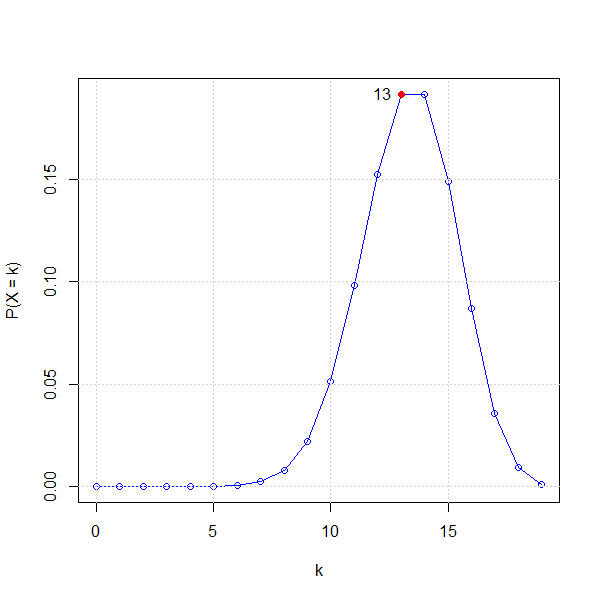
\includegraphics[width=0.5\linewidth]{3.21.png}
\end{figure}
用R语言模拟,标注的最大值点为$13$,而$14$未被标注的原因涉及到舍入误差(数值分析).
\begin{lstlisting}
# 设置二项分布的参数
n <- 19 p <- 0.7
# 设置数字的显示精度为 15 位
options(digits = 15)
# 计算 k=13 和 k=14 对应的概率
probability_k13 <- dbinom(13, size = n, prob = p)
probability_k14 <- dbinom(14, size = n, prob = p)
# 打印结果
cat("P(X=13) =", probability_k13, "\n")
cat("P(X=14) =", probability_k14, "\n")
\end{lstlisting}
结果显示$P(X=13)=0.191638982753443$,$P(X=14)=0.191638982753442$.

绘制图象的代码如下:
\begin{lstlisting}
# 设置二项分布的参数
n <- 19 p <- 0.7
# 创建一个包含可能的 k 值的向量
k_values <- 0:n
# 计算每个 k 对应的概率
probabilities <- dbinom(k_values, size = n, prob = p)
# 找到所有概率最大的 k 值
max_prob <- max(probabilities)
max_k_values <- k_values[probabilities == max_prob]
# 创建数据框
result_table <- data.frame(k = k_values, probability = probabilities)
# 绘制概率分布图,并在图上标注最大概率点
plot(k_values, probabilities, type = "o", xlab = "k", ylab = "P(X = k)", col = "blue")
points(max_k_values, rep(max_prob, length(max_k_values)), col = "red", pch = 19)
text(max_k_value, max(probabilities), labels = max_k_value, pos = 2)
grid()
# 打印表格
print(result_table)
\end{lstlisting}
3.22 全班有$95$个学生,每个学生上课迟到的概率为$p$.假设每个学生是否迟到是相互独立的.

(a)当$p=0.05$时,有多少个学生迟到的概率最大;

(b)如果有$7$个人迟到,你认为$p$是多少?
\begin{solution}
设迟到的学生数为随机变量$X$,则$X\sim B(95,p)$

(a)当$p=0.05$时,有
\[{p_k} = P(X = k) = C_{95}^k{0.05^k}{0.95^{95 - k}}\]
是$k$的函数,于是有
\[{p_{k + 1}} - {p_k} = C_{95}^{k + 1}{0.05^{k + 1}}{0.95^{95 - (k + 1)}} - C_{95}^k{0.05^k}{0.95^{95 - k}} = \frac{{95!}}{{k!(94 - k)!}}{0.05^k}{0.95^{95 - (k + 1)}}\left( {\frac{{0.05}}{{k + 1}} - \frac{{0.95}}{{95 - k}}} \right)\]
判断单调性可得
\[\frac{{0.05}}{{k + 1}} - \frac{{0.95}}{{95 - k}} > 0 \Rightarrow 3.8 > k\]
这表明$k\leqslant 3$时$p_k$递增,$k\geqslant 4$时$p_k$递减,此时$p_4-p_3>0$,故最大值点为$k=4$,即$4$个学生迟到的概率最大.

(b)即求$p$使得,$P(X=7)$最大
\[P(X = 7) = C_{95}^7{p^7}{(1 - p)^{88}}\]
是$p$的函数,记作$f(p)$,求导可得
\[f'(p) = C_{95}^7{p^6}{(1 - p)^{87}}(7 - 95p)\]
这表明$p=\frac{7}{95}$时,迟到$7$个人的概率最大.
\end{solution}
\begin{figure}[H]
    \centering
    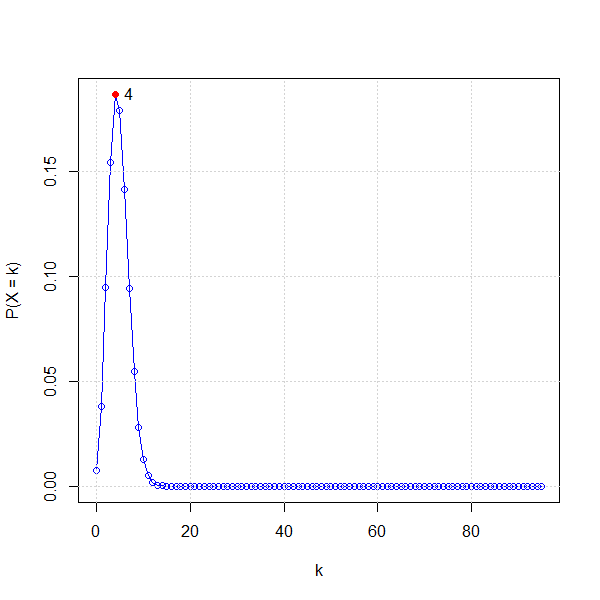
\includegraphics[width=0.5\linewidth]{3.22.png}
\end{figure}
依旧用R语言模拟,对参数微调即可,故这里不再给出代码.
\begin{remark}
结合3.21和3.22我们来考虑一般的情形,设$X\sim B(n,p)$,则有
\[{P_{k + 1}} - {P_k} = C_n^{k + 1}{p^{k + 1}}{(1 - p)^{n - (k + 1)}} - C_n^k{p^k}{(1 - p)^{n - k}}\]
整理得到
\[{P_{k + 1}} - {P_k} = \frac{{n!}}{{k!(n - k - 1)!}}{p^k}{(1 - p)^{n - (k + 1)}}\left( {\frac{p}{{k + 1}} - \frac{{1 - p}}{{n - k}}} \right)\]
判断单调性可得
\[\frac{p}{{k + 1}} - \frac{{1 - p}}{{n - k}} > 0 \Rightarrow np - kp > k + 1 - kp - p \Rightarrow (n + 1)p - 1 > k\]
这就得到了已知$n,p$情形下的最值点,最值点应为$[(n + 1)p - 1] + 1$,若$(n + 1)p - 1$已为整数,则有两个最值点.

如果要求使得$P(X=k)$最大的$p$,则记
\[f(p) = C_n^k{p^k}{(1 - p)^{n - k}}\]
于是有
\[f'(p) = C_n^k{p^{k - 1}}{(1 - p)^{n - k - 1}}\left( {k(1 - p) - (n - k)p} \right) = C_n^k{p^{k - 1}}{(1 - p)^{n - k - 1}}(k - np)\]
这表明使得$P(X=k)$最大的$p$等于$\frac{k}{n}$.
\end{remark}

3.23 设$X$是服从参数是$\lambda$的Poisson分布.

(a)已知$\lambda=23.8$,求$p_k=P(X=k)$的最大值点$k$;

(b)已知$X=21$,求使得$P(X=21)$达到最大的$\lambda$.
\begin{solution}

(a)$X\sim P(23.8)$,于是有
\[{p_k} = P(X = k) = \frac{{{{23.8}^k}}}{{k!}}{e^{ - 23.8}}\]
是关于$k$的函数,于是有
\[{p_{k + 1}} - {p_k} = \frac{{{{23.8}^{k + 1}}}}{{(k + 1)!}}{e^{ - 23.8}} - \frac{{{{23.8}^k}}}{{k!}}{e^{ - 23.8}} = \frac{{{{23.8}^k}}}{{k!}}{e^{ - 23.8}}\left( {\frac{{23.8}}{{k + 1}} - 1} \right)\]
判断单调性可得
\[\frac{{23.8}}{{k + 1}} - 1 > 0 \Rightarrow 22.8 > k\]
这表明$k\leqslant 22$时$p_k$递增,$k\geqslant 23$时$p_k$递减,此时$p_{23}-p_{22}>0$,故最大值点为$k=23$.

(b)即求$\lambda$使得,$P(X=21)$最大
\[P(X = 21) = \frac{{{\lambda ^{21}}}}{{21!}}{e^{ - \lambda }}\]
是$\lambda$的函数,记作$f(\lambda)$,求导可得
\[f'(\lambda ) = \frac{{21{\lambda ^{20}}}}{{21!}}{e^{ - \lambda }} - \frac{{{\lambda ^{21}}}}{{21!}}{e^{ - \lambda }} = \frac{{{\lambda ^{20}}}}{{21!}}{e^{ - \lambda }}\left( {21 - \lambda } \right)\]
这表明$\lambda=21$时,$P(X=21)$达到最大.
\end{solution}
绘图代码如下
\begin{lstlisting}
# 设置参数
lambda <- 23.8
# 计算概率质量函数
pk <- function(k) {exp(-lambda) * (lambda^k) / factorial(k)}
# 创建一个包含可能的 k 值的向量
k_values <- 0:50
# 计算每个 k 对应的概率
probabilities <- sapply(k_values, pk)
# 找到概率最大的 k 值
max_prob_index <- which.max(probabilities)
max_k <- k_values[max_prob_index]
# 绘制概率质量函数图像,并在图上标注最大概率点
plot(k_values, probabilities, type = "o", xlab = "k", ylab = "P(X = k)", col = "blue")
points(max_k, probabilities[max_prob_index], col = "red", pch = 19)
text(max_k_value, max(probabilities), labels = max_k, pos = 2)
grid()
\end{lstlisting}
\begin{figure}[H]
    \centering
    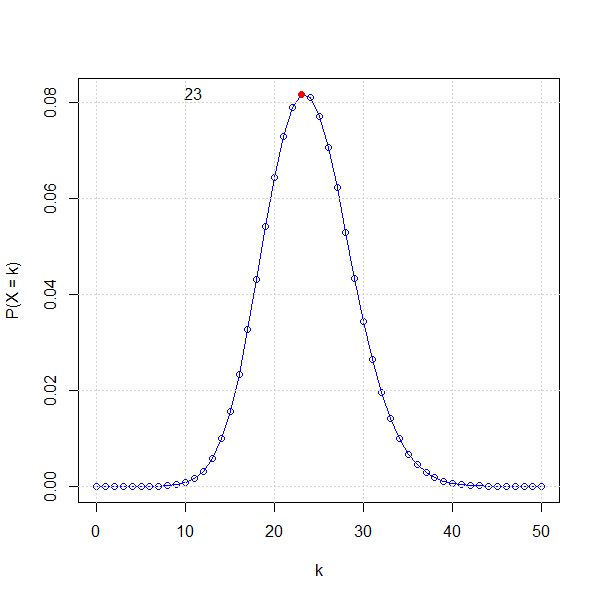
\includegraphics[width=0.5\linewidth]{3.23.png}
\end{figure}
\begin{remark}
结合3.23我们来考虑一般的情形,设$X\sim P(\lambda)$,则有
\[{P_{k + 1}} - {P_k} = \frac{{{\lambda ^{k + 1}}}}{{(k + 1)!}}{e^{ - \lambda }} - \frac{{{\lambda ^k}}}{{k!}}{e^{ - \lambda }} = \frac{{{\lambda ^k}}}{{k!}}{e^{ - \lambda }}\left( {\frac{\lambda }{{k + 1}} - 1} \right)\]
判断单调性可得
\[\frac{\lambda }{{k + 1}} - 1 > 0 \Rightarrow \lambda  - 1 > k\]
这就得到了已知$\lambda$情形下的最值点,最值点应为$[\lambda - 1] + 1$,若$ \lambda - 1$已为整数,则有两个最值点.

如果要求使得$P(X=k)$最大的$\lambda$,则记
\[f(\lambda ) = \frac{{{\lambda ^k}}}{{k!}}{e^{ - \lambda }}\]
于是有
\[f'(\lambda ) = \frac{{k{\lambda ^{k - 1}}}}{{k!}}{e^{ - \lambda }} - \frac{{{\lambda ^k}}}{{k!}}{e^{ - \lambda }} = \frac{{{\lambda ^k}}}{{k!}}{e^{ - \lambda }}\left( {k - \lambda } \right)\]
这表明使得$P(X=k)$最大的$\lambda$恰为$k$.
\end{remark}

3.24 假设你每天收到的短信数服从参数是$\lambda$的Poisson分布.

(a)已知$\lambda=8.9$时,你今天收到多少个短信的概率最大?

(b)如果你今天收到了$12$个短信,你认为$\lambda$应当是多少?
\begin{solution}
根据3.23和上面的注记,易知(a)$k=8$;(b)$\lambda=12$
\end{solution}

3.25 将一个骰子投掷$n$次,用$m$表示掷得的最小点数,用$M$表示掷得的最大点数,计算:

(a)$P(m=k),1\leqslant k\leqslant 6$;

(b)$P(M=k),1\leqslant k\leqslant 6$;

(c)$P(m=2,M=5)$.
\begin{solution}
(a)由于\[P(m = k) = P(m \geqslant k) - P(m \geqslant k + 1)\]
记第$i$次投掷的最小点数为$m_i$,则有
\[P(m \geqslant k) = P({m_1} \geqslant k,{m_2} \geqslant k, \cdots ,{m_n} \geqslant k)\]
由于每次投掷骰子相互独立,故
\[P(m \geqslant k) = P({m_1} \geqslant k)P({m_2} \geqslant k) \cdots P({m_n} \geqslant k) = {\left( {\frac{{7 - k}}{6}} \right)^n}\]
于是得到
\[P(m = k) = P(m \geqslant k) - P(m \geqslant k + 1) = {\left( {\frac{{7 - k}}{6}} \right)^n} - {\left( {\frac{{6 - k}}{6}} \right)^n}\]

(b)由于
\[P(M = k) = P(M \leqslant k) - P(M \leqslant k - 1)\]
记第$i$次投掷的最大点数为$M_i$,则有
\[P(M \leqslant k) = P({M_1} \leqslant k,{M_2} \leqslant k, \cdots ,{M_n} \leqslant k)\]
由于每次投掷骰子相互独立,故
\[P(M \leqslant k) = P({M_1} \leqslant k)P({M_2} \leqslant k) \cdots P({M_n} \leqslant k) = {\left( {\frac{k}{6}} \right)^n}\]
于是得到
\[P(M = k) = P(M \leqslant k) - P(M \leqslant k - 1) = {\left( {\frac{k}{6}} \right)^n} - {\left( {\frac{{k - 1}}{6}} \right)^n}\]

(c)记$n$次投掷出现过的点数为$X$,则
\[P(m = 2,M = 5) = P(2 \leqslant X \leqslant 5) - P(2 \leqslant X \leqslant 4) - P(3 \leqslant X \leqslant 5) + P(3 \leqslant X \leqslant 4)\]
计算可得
\[P(m = 2,M = 5) = \frac{{{4^n} - 2 \cdot {3^n} + {2^n}}}{{{6^n}}} = {\left( {\frac{2}{3}} \right)^n} - 2 \cdot {\left( {\frac{1}{2}} \right)^n} + {\left( {\frac{1}{3}} \right)^n}\]
\end{solution}
\begin{remark}
3.25(c)计算非$m=2,M=5$的情形时,实际上用到了加法公式,即$P(m \geqslant 3,M \leqslant 5 \cup m \geqslant 2,M \leqslant 4)$,如果引入新的随机变量$X$,则可以像上面的解法一样省略这一过程(本质上还是一样的).
\end{remark}

3.26 设点随机地落在中心在原点,半径为$R$的圆周上.求落点横坐标的概率密度.
\begin{solution}
设落点的横坐标为随机变量$X$,作极坐标变换则有$X=R\cos \theta$,由于点随机地落在圆周上,因此$\theta\sim U(0,2\pi)$.此时$P(X\in (-R,R))=1$,于是有
\[P(X = x) = P(R\cos \theta  = x) = P(\theta  = \arccos \frac{x}{R}) + P(\theta  = 2\pi  - \arccos \frac{x}{R})\]
将$\theta$的密度函数代入可得
\[P(X = x) = \frac{1}{{2\pi }}\frac{1}{{R\sqrt {1 - \frac{{{x^2}}}{{{R^2}}}} }}dx + \frac{1}{{2\pi }}\frac{1}{{R\sqrt {1 - \frac{{{x^2}}}{{{R^2}}}} }}dx = \frac{1}{{\pi \sqrt {{R^2} - {x^2}} }}dx\]
这表明$X$有概率密度
\[{f_X}(x) = \frac{1}{{\pi \sqrt {{R^2} - {x^2}} }},x \in ( - R,R)\]
\end{solution}

3.27 某人在等待一个朋友的消息,如果从任何时间$t$开始,在充分小的时间段$(t,t+s]$内得到他朋友的消息的概率与$s$成正比,计算等待时间服从的分布.
\begin{solution}
记某人等待朋友消息的等待时间为随机变量$X$,$X$的分布函数为$F(t)$,概率密度为$f(t)$,根据题意当$s$充分小时,有
    \[P(t < X \leqslant t + s|X>t) = \lambda s,\lambda  > 0\]
于是得到
    \[\lambda s = \frac{{P(t < X \leqslant t + s)}}{{P(X>t)}} = \frac{{F(t + s) - F(t)}}{{1 - F(t)}}\]
由$s$充分小,移项取极限可得
    \[\lambda  = \frac{1}{{1 - F(t)}}\mathop {\lim }\limits_{s \to 0} \frac{{F(t + s) - F(t)}}{s} \Rightarrow \lambda  = \frac{{f(t)}}{{1 - F(t)}}\]
这是一个变量分离方程,积分可得
    \[-\ln (1 - F) = \lambda t + C \Rightarrow F = 1 - C{e^{-\lambda t}}\]
根据初值归一化条件可得$C=1$,这表明等待时间服从指数分布.
\end{solution}
\begin{remark}
3.27与3.14并无本质区别.
\end{remark}

3.28 设$X$有概率密度$f(x)=cx/\pi^2,x\in (0,\pi)$.求$Y=\sin X$的概率密度.
\begin{solution}
由归一化条件可得
\[1 = \int_{ - \infty }^\infty  {f(x)dx}  = \int_0^\pi  {\frac{{cx}}{{{\pi ^2}}}dx}  \Rightarrow c = 2\]
由于$x\in (0,\pi)$,故$P(Y\in (0,1))=1$,划分分段单调区间可得,在$(0,\frac{\pi}{2}]$上$X=\arcsin Y$,在$(\frac{\pi}{2},\pi)$上,$X=\pi-\arcsin Y$,于是有
\[P(Y = y) = P(\sin X = y) = P(X = \arcsin y) + P(X = \pi  - \arcsin y)\]
将密度函数代入可得
\[P(Y = y) = \frac{{2\arcsin y}}{{{\pi ^2}}}\frac{1}{{\sqrt {1 - {y^2}} }}dy + \frac{{2(\pi  - \arcsin y)}}{{{\pi ^2}}}\frac{1}{{\sqrt {1 - {y^2}} }}dy = \frac{2}{{\pi \sqrt {1 - {y^2}} }}dy\]
这表明$Y$有密度函数
\[{f_Y}(y) = \frac{2}{{\pi \sqrt {1 - {y^2}} }},y\in(0,1)\]
\end{solution}
\begin{remark}
3.28需要用到数学分析中的知识:严格单调的连续函数必有严格单调的反函数.另外还需要注意微分法要求$D$为开集.
\end{remark}

3.29 设$X \sim  U(0,1)$,$\Phi^{-1}(x)$是$\Phi(x)$的反函数,求$Y=\Phi^{-1} (X)$的分布函数.
\begin{solution}
由于$X\sim U(0,1)$,故$f_X(x)=1,x\in(0,1)$,由于$\Phi(y)\in (0,1)$,于是有
    \[P(Y=y)=P(X=\Phi(y))=f_X(\Phi(y))d(\Phi(y))=\varphi(y)dy\]
这表明$Y\sim N(0,1)$.
\end{solution}
\newpage
3.30 设$f(x)$是$[0,\infty)$中的连续函数.

(1)如果任取$x,y>0$,有$f(x+y)=f(x)+f(y)$,则有常数$a$使得$f(x)=ax,x\geqslant 0$;

(2)如果任取$x,y>0$,有$g(x+y)=g(x)\cdot g(y)>0$,则有常数$b$使得$g(x)=e^{bx},x\geqslant 0$.
\begin{solution}
(1)取$y=x$,则$f(2x)=2f(x)$,不妨设$f[(n-1)x]=(n-1)f(x)$,则有
\[f(nx) = f[(n - 1)x + x] = f[(n - 1)x] + f(x) = (n - 1)f(x) + f(x) = nf(x)\]
于是得到$f(nx)=nf(x)$,对于$n\in \mathbb{N}^+$成立.

取$x=x/n,n\in \mathbb{N}^+$,有
\[f(x) = nf(\frac{x}{n}) \Rightarrow f(\frac{x}{n}) = \frac{1}{n}f(x)\]
故对于正有理数$m/n(m,n\in \mathbb{N}^+)$,成立
\[f(\frac{m}{n}) = \frac{m}{n}f(1)\]
于是对于任意的有理数已成立$f(x)=f(1)x$,只需验证对无理数也成立即可,根据实数的连续性(完备性),任何无理数总可以用有理数列逼近,$\forall x\in [0,\infty)$,存在有理数列$\{x_n\}$收敛至$x$,根据Heine定理,有
\[\mathop {\lim }\limits_{n \to \infty } f({x_n}) = f(x)\]
于是有
\[f(x) = \mathop {\lim }\limits_{n \to \infty } f({x_n}) = \mathop {\lim }\limits_{n \to \infty } {x_n}f(1) = f(1)x\]
(2)取$f(x)=\ln g(x)$,则
\[g(x + y) = {e^{f(x + y)}} = {e^{f(x) + f(y)}} = {e^{f(x)}} \cdot {e^{f(y)}} = g(x) \cdot g(y)\]
由(1)知$f(x)=f(1)x$,于是有
\[g(x) = {e^{f(1)x}}\]
\end{solution}
\begin{remark}
3.30题完全是数学分析中的问题(函数方程的连续解),在谢惠民、裴礼文等著名的数学分析习题集上都能找到,原问题只要求$f(x)$在$0$一点连续,就可证满足$f(x+y)=f(x)+f(y)$的函数在$\mathbb{R}$上连续,且$f(x)=f(1)x$.
\end{remark}
\begin{remark}
3.30(1)我们进一步加强条件,若$f(x)$在$[0,\infty)$可微,将$x=1/n$代入$f(nx)=nf(x)$可得
\[f(1) = nf(\frac{1}{n}),\forall n{ \in \mathbb{N}^ + }\]
由于$f(x)$在$[0,\infty)$上连续,故
\[f(1) = \mathop {\lim }\limits_{n \to \infty } nf(\frac{1}{n}) \Rightarrow \mathop {\lim }\limits_{n \to \infty } f(\frac{1}{n}) = 0 \Rightarrow f(0) = 0\]
于是有
\[f'(0) = \mathop {\lim }\limits_{\Delta x \to 0} \frac{{f(\Delta x) - f(0)}}{{\Delta x}} = \mathop {\lim }\limits_{\Delta x \to 0} \frac{{f(\Delta x)}}{{\Delta x}}\]
将$y=\Delta x$代入可得
\[f(x + \Delta x) = f(x) + f(\Delta x) \Rightarrow \mathop {\lim }\limits_{\Delta x \to 0} \frac{{f(x + \Delta x) - f(x)}}{{\Delta x}} = \mathop {\lim }\limits_{\Delta x \to 0} \frac{{f(\Delta x)}}{{\Delta x}}\]
这表明$f'(x)=f'(0)$,记$f'(0)=a$,则有$f(x)=ax+C$,将初值$f(0)=0$代入可得$C=0$,故
\[f(x) = ax,a \geqslant 0\]
上面的方法是ODE中求解函数方程的方法.
\end{remark}

3.31 设$X$服从参数为$\lambda$的指数分布,求
\[Y = \left\{ \begin{gathered}
  X \hfill \quad X\geqslant 1\\
  {X^2} \hfill \quad  X<1\\ 
\end{gathered}  \right.\]

的概率密度.
\begin{solution}
取开集$D=(0,+\infty)$
    \[P(Y\in D)=P(Y>1)+P(Y\in (0,1))=P(X>1)+P(X^2\in (0,1))=1\]
由于$X\sim \varepsilon(\lambda)$,因此对$y>1$有
    \[P(Y = y) = P(X = y) = \lambda {e^{ - \lambda y}}dy\]
对$y\in (0,1)$有
\[P(Y = y) = P({X^2} = y) = P(X = \sqrt y ) = \lambda {e^{ - \lambda \sqrt y }}d\sqrt y  = \frac{{\lambda {e^{ - \lambda \sqrt y }}}}{{2\sqrt y }}dy\]
于是得到$Y$的概率密度
    \[{f_Y}(y) = \left\{ \begin{gathered}
  \lambda {e^{ - \lambda y}} \hfill \quad y>1\\
  \frac{{\lambda {e^{ - \lambda \sqrt y }}}}{{2\sqrt y }} \hfill \quad y\in(0,1)\\ 
\end{gathered}  \right.\]
\end{solution}

\newpage
\section{随机向量}
4.1 设随机向量$(X,Y)$有联合分布函数



4.3 设离散型概率分布$p_{ij}=P(X=i,Y=j)$如下表所示

\begin{table}[ht]
    \centering
    \begin{tabular}{|c|c|c|c|c|c|} \hline 
 $p_{ij}$&  $1$&$2$&$3$&$4$&$5$\\ \hline 
 $1$&  $0.06$&$0.05$    &$0.04$&$0.01$&$0.02$\\ \hline 
         $2$&    $0.05$&$0.10$&$0.10$&$0.05$&$0.03$\\ \hline 
         $3$& 
      $0.07$&$0.05$& $0.01$&$0.02$&$0.02$\\ \hline
 $4$& $0.05$& $0.02$& $0.01$&$0.01$&$0.03$\\\hline
 $5$& $0.05$& $0.06$& $0.05$& $0.02$&$0.02$\\\hline\end{tabular}
\end{table}

(1)求$X,Y$的边缘分布;
\begin{solution}
\begin{table}[ht]
    \centering
    \begin{tabular}{|c|c|c|c|c|c|} \hline 
         $X$&  $1$& $2$&$3$& $4$&$5$\\ \hline 
         $P$& 
     $0.18$& $0.33$& $0.17$& $0.12$&$0.20$\\ \hline\end{tabular}

\end{table}
    \begin{table}[ht]
    \centering
    \begin{tabular}{|c|c|c|c|c|c|} \hline 
         $Y$&  $1$& $2$&$3$& $4$&$5$\\ \hline 
         $P$& 
     $0.28$& $0.28$& $0.21$& $0.11$&$0.12$\\ \hline\end{tabular}

\end{table}

\end{solution}
(2)求$U=\max(X,Y)$的分布;
\begin{solution}
    
\begin{table}[H]
    \centering
    \begin{tabular}{|c|c|c|c|c|c|} \hline 
         $U$ & 1 & 2 & 3 & 4 & 5 \\ \hline 
         $P$ & 0.06 & 0.20 & 0.27 & 0.17 & 0.30 \\ \hline
    \end{tabular}
\end{table}

\end{solution}

(3)求$V=\min(X,Y)$的分布;

\begin{solution}
       \begin{table}[H]
    \centering
    \begin{tabular}{|c|c|c|c|c|c|} \hline 
         $U$&  $1$& $2$&$3$& $4$&$5$\\ \hline 
         $P$& 
     $0.40$& $0.41$& $0.11$& $0.06$&$0.02$\\ \hline\end{tabular}
\end{table}

\end{solution}

(4)计算$P(X=2|Y=3)$
\begin{solution}
    \[P(X=2|Y=3)=\frac{P(X=2,Y=3)}{P(Y=3)}=\frac{10}{21}\]
\end{solution}

4.6 设$X\sim B(n,p),Y\sim B(m,p)$,当$X,Y$独立,计算$X+Y$的概率分布.
\begin{solution}
\[P(X + Y = k) = \sum\limits_{i = 0}^k {P(X = i,Y = k - i)} \]
由$X,Y$独立可得
\[\sum\limits_{i = 0}^k {P(X = i,Y = k - i)}  = \sum\limits_{i = 0}^k {P(X = i)P(Y = k - i)} \]
于是有
\[P(X + Y = k) = \sum\limits_{i = 0}^k {C_n^i{p^i}{{(1 - p)}^{n - i}}C_m^{k - i}{p^{k - i}}{{(1 - p)}^{m - k + i}}}  = \sum\limits_{i = 0}^k {C_n^iC_m^{k - i}{p^k}{{(1 - p)}^{n + m - k}}} \]
于是得到
\[P(X + Y = k) = C_{n + m}^k{p^k}{(1 - p)^{n + m - k}}\]
这表明$X+Y\sim B(n+m,p)$.
\end{solution}

4.8 如果随机向量$(X,Y)$有如下概率分布:
\[
P(X=i,Y=\frac{1}{i})=c,i=1,2,\cdots,8
\]
确定常数$c$并求$X,Y$的概率分布.
\begin{solution}
    \[\sum\limits_{i = 1}^8 {P(X = i,Y = \frac{1}{i})}  = 1 \Rightarrow c = \frac{1}{8}\]
    于是得到$X,Y$的概率分布为
    \[P(X = i) = \frac{1}{8},P(Y = \frac{1}{i}) = \frac{1}{8},i = 1,2, \cdots ,8\]
\end{solution}

4.9 设随机变量$X,Y$独立同分布,证明
\[
P(a<\min (X,Y)\leqslant b)=P^2(X>a)-P^2(X>b)
\]
\begin{myproof}
   \[P(a < \min (X,Y) \leqslant b) = P(\min (X,Y) > a) - P(\min (X,Y) > b) = P(X > a,Y > a) - P(X > b,Y > b)\]
    由于$X,Y$独立因此可以得到
    \[P(X > a,Y > a) - P(X > b,Y > b) = P(X > a)P(Y > a) - P(X > b)P(Y > b)\]
    再由$X,Y$同分布可以得到
    \[P(a < \min (X,Y) \leqslant b) = {P^2}(X > a) - {P^2}(X > b)\]
\end{myproof}

4.15 设随机向量$(X,Y)$有联合密度
\[f(x,y) = \left\{ \begin{gathered}
  {e^{ - x}} \hfill \quad 0<y<x\\
  0 \hfill \quad \text{其他}\\ 
\end{gathered}  \right.\]
求$X,Y$的边缘密度.
\begin{solution}
\[{f_X}(x) = \int_0^x {{e^{ - x}}dy}  = x{e^{ - x}}\]
    \[{f_Y}(y) = \int_y^\infty  {{e^{ - x}}dx}  = {e^{ - y}}\]
\end{solution}

4.16 设$p=1-q\in (0,1)$,$0<\alpha<q/p$.假设一个家庭有$n$个小孩的概率是
\[{p_n} = \left\{ \begin{gathered}
  \alpha {p^n} \hfill \quad n\geqslant 1\\
  1 - \alpha p/q \hfill \quad n=0\\ 
\end{gathered}  \right.\]
如果男孩和女孩的出生是等可能的,求一个家庭有$k$个男孩的概率.
\begin{solution}
用$X$表示一个家庭的男孩个数,$Y$表示一个家庭的小孩数.    
\[P(X = k) = P(Y = n)P(X = k|Y = n)\]
    (i)$k=0$时,根据全概率公式
    \[P(X = 0) = 1 - \alpha \frac{p}{q} + {\sum\limits_{n = 1}^\infty  {\alpha {p^n}\left( {\frac{1}{2}} \right)} ^n} = 1 - \alpha \frac{p}{q} + \alpha \frac{{\frac{p}{2}}}{{1 - \frac{p}{2}}} = 1 - \frac{{\alpha p}}{q} + \frac{{\alpha p}}{{2 - p}}\]
    (ii)$k\geqslant 1$时,根据全概率公式
    \[P(X = k) = \alpha {\sum\limits_{n = k}^\infty  {C_n^k\left( {\frac{p}{2}} \right)} ^n} = \alpha {\sum\limits_{m = 0}^\infty  {C_{m + k}^k\left( {\frac{p}{2}} \right)} ^{m + k}} = \alpha {\left( {1 - \frac{p}{2}} \right)^{ - (k + 1)}}{\left( {\frac{p}{2}} \right)^k}\]
\end{solution}

4.17 同课件习题$5$

4.22 设随机变量$X,Y$独立,$X$有概率密度$f(x)$,$Y$有离散型概率分布$P(Y=a_i)=p_i>0,i=1,2,\cdots$,若$a_i$均不为零,证明$Z=XY$有概率密度
\[h(z) = \sum\limits_{i = 1}^\infty  {\frac{{{p_i}}}{{|{a_i}|}}f\left( {\frac{z}{{{a_i}}}} \right)} \]
\begin{myproof}
 $P(Z=z)=P(XY=z)$
 由于$a_i\ne 0$,根据全概率公式
\[P(XY = z) = \sum\limits_{i = 1}^\infty  {P(Y = {a_i})P(XY = z|Y = {a_i})}  = \sum\limits_{i = 1}^\infty  {P(Y = {a_i})P(X = \frac{z}{{{a_i}}})} \]
根据微分法
\[P(X = \frac{z}{{{a_i}}}) = f\left( {\frac{z}{{{a_i}}}} \right)\frac{1}{{|{a_i}|}}dz\]
于是得到
\[P(XY = z) = \sum\limits_{i = 1}^\infty  {\frac{{{p_i}}}{{|{a_i}|}}f\left( {\frac{z}{{{a_i}}}} \right)dz} \]
即
\[h(z) = \sum\limits_{i = 1}^\infty  {\frac{{{p_i}}}{{|{a_i}|}}f\left( {\frac{z}{{{a_i}}}} \right)} \]
\end{myproof}

4.25 设随机变量$U$和$V$独立,都服从$(0,1)$上的均匀分布.

(a)计算$r=\sqrt{-2\ln U}$和$\theta=2\pi V$的概率密度.

(b)证明$X=r\cos(\theta),Y=r\sin(\theta)$独立,都服从标准正态分布.

\begin{solution}
(a)\[
P(r=x)=P(\sqrt{-2\ln U}=x)=P(U=e^{-\frac{x^2}{2}})=xe^{-\frac{x^2}{2}}dx
\]
\[
P(\theta=y)=P(2\pi V=y)=P(V=\frac{y}{2\pi })=\frac{1}{2\pi}dy
\]
于是得到概率密度
\[f(r) = \left\{ \begin{gathered}
    x{e^{ - \frac{{{x^2}}}{2}}} \hfill \quad x\in (0,\infty)\\
  0 \hfill \quad \text{其他}\\ 
\end{gathered}  \right.,f(\theta)  = \left\{ \begin{gathered}
  \frac{1}{{2\pi }} \hfill  \quad x\in (0,2\pi)\\
  0 \hfill \quad \text{其他}\\ 
\end{gathered}  \right.\]
(b)
\[
P(X=x,Y=y)=P(r\cos(\theta)=x,r\sin(\theta)=y)=P(r=\sqrt{x^2+y^2},\theta=\arctan(\frac{y}{x}))
\]
\[{J^ - }^1 = \left| {\begin{array}{*{20}{c}}
  {\cos \theta }&{ - r\sin \theta } \\ 
  {\sin \theta }&{r\cos \theta } 
\end{array}} \right| = r\]
于是有
\[P(X = x,Y = y) = P(r = \sqrt {{x^2} + {y^2}} ,\theta  = \arctan (\frac{y}{x})) =   \sqrt {{x^2} + {y^2}} {e^{ - \frac{{{x^2} + {y^2}}}{2}}}\frac{1}{{2\pi }}\frac{1}{{\sqrt {{x^2} + {y^2}} }}dxdy\]
可得联合密度
\[f(x,y) = \frac{1}{{2\pi }}{e^{ - \frac{{{x^2} + {y^2}}}{2}}}\]
积分计算边缘分布
\[{f_X}(x) = \int_{ - \infty }^\infty  {{e^{ - \frac{{{x^2} + {y^2}}}{2}}}} dy = \frac{1}{{\sqrt {2\pi } }}{e^{ - \frac{{{x^2}}}{2}}},{f_Y}(y) = \int_{ - \infty }^\infty  {{e^{ - \frac{{{x^2} + {y^2}}}{2}}}} dx = \frac{1}{{\sqrt {2\pi } }}{e^{ - \frac{{{y^2}}}{2}}}\]
这表明$X,Y$独立,且都服从标准正态分布.
\textcolor{red}{联合密度可以拆分为乘积形式已经可以说明独立.}
\end{solution}

4.30 设随机变量$X,Y$独立,$X\sim \mathscr{E}(\lambda),Y\sim \mathscr{E}(\mu)$.分别求$U=\min (X,Y),V=\max(X,Y),W=X/Y$的概率密度.
\begin{solution}
    \[f_X(x)=\lambda e^{-\lambda x},f_Y(y)=\mu e^{-\mu y}\]
    由$X,Y$独立可得联合密度
\[f(x,y) = f(x)f(y) = \lambda \mu {e^{ - (\lambda x + \mu y)}},x > 0,y > 0\]
    先求$U,V$的联合密度,$P(v>u)=1$
\[P(U = u,V = v) = P(X = u,Y = v) + P(X = v,Y = u) = \lambda \mu {e^{ - (\lambda u + \mu v)}} + \lambda \mu {e^{ - (\lambda v + \mu u)}}dvdu\]
于是得到
\[f(u,v) = \lambda \mu ({e^{ - (\lambda u + \mu v)}} + {e^{ - (\lambda v + \mu u)}}).u > 0,v > 0\]
计算边缘密度可得
\[f(u) = \int_u^\infty  {\lambda \mu ({e^{ - (\lambda u + \mu v)}} + {e^{ - (\lambda v + \mu u)}})dv}  = (\lambda  + \mu ){e^{ - (\lambda  + \mu )u}}\]
\[f(v) = \int_0^v {\lambda \mu ({e^{ - (\lambda u + \mu v)}} + {e^{ - (\lambda v + \mu u)}})du}  = \lambda {e^{ - \lambda v}} + \mu {e^{ - \mu v}} - (\lambda  + \mu ){e^{ - (\lambda  + \mu )v}}\]
计算$(Y,W)$的联合密度
\[
P(Y=y,W=w)=P(Y=y,\frac{X}{Y}=w)=P(X=yw,Y=y)
\]
\[|{J^{ - 1}}| = \left| {\begin{array}{*{20}{c}}
  {\frac{1}{y}}&{ - \frac{x}{{{y^2}}}} \\ 
  0&1 
\end{array}} \right| = \frac{1}{y} \Rightarrow J = y\]
    于是得到
    \[P(Y = y,W = w) = \lambda \mu {e^{ - (\lambda w + \mu )y}}ydwdy\]
    积分计算$W$的边缘密度得到
    \[f(w) = \lambda \mu \int_0^\infty  {y{e^{ - (\lambda w + \mu )y}}} dy = 0 + \frac{{\lambda \mu }}{{\lambda w + \mu }}\int_0^\infty  {{e^{ - (\lambda w + \mu )y}}} dy = \frac{{\lambda \mu }}{{{{(\lambda w + \mu )}^2}}}\]
    
\end{solution}

4.34 设随机变量$X\sim \mathscr{E}(1),Y\sim \mathscr{E}(1)$,$X,Y$独立,$U=X^2+Y^2,V=X^2/Y^2$.求$(U,V)$的联合密度.
\begin{solution}
    $X$与$Y$同分布,有相同的分布函数$e^{-t}$,$P(x>0,y>0)=1$,可得联合密度
    \[f(x,y) = f(x)f(y) = {e^{ - (x + y)}},(x>0,y>0)\]
    
    $P(u>0,v>0)=1$于是得到
   \[P(U = u,V = v) = P({X^2} + {Y^2} = u,\frac{{{X^2}}}{{{Y^2}}} = v) = P(X =  \sqrt {\frac{{uv}}{{v + 1}}} ,Y =   \sqrt {\frac{u}{{v + 1}}} )\]
 \[|{J^{ - 1}}| = \left| {\begin{array}{*{20}{c}}
  {2x}&{2y} \\ 
  {\frac{{2x}}{{{y^2}}}}&{\frac{{ - 2{x^2}}}{{{y^3}}}} 
\end{array}} \right| = \left| {\frac{{ - 4{x^3}}}{{{y^3}}} - \frac{{4x}}{y}} \right| \Rightarrow |J| = \left| {\frac{1}{{4\sqrt{v}(1 + v))}}} \right|\]
于是得到
\[P(U = u,V = v) = {e^{ - (\sqrt {\frac{{uv}}{{v + 1}}}  + \sqrt {\frac{u}{{v + 1}}} )}}\frac{1}{{4\sqrt{v}(1 + v)}}dudv\]
因此有联合密度
\[f(u,v) = {e^{ - (\sqrt {\frac{{uv}}{{v + 1}}}  + \sqrt {\frac{u}{{v + 1}}} )}}\frac{1}{{4\sqrt{v}(1 + v)}},u > 0,v > 0\]
\end{solution}

4.36 证明如果随机向量$(X,Y)$有联合密度$f(x,y)$,$(U,V)$由线性变换
\[
\left(\begin{array}{cc}
     U \\
      V
\end{array}\right)=A\left(\begin{array}{cc}
     X \\
      Y
\end{array}\right)
\]
决定,其中
\[
A=\left(\begin{array}{cc}
     a &b \\
      c& d
\end{array}\right),A^{-1}=\left(\begin{array}{cc}
     a_1 &b_1 \\
      c_1& d_1
\end{array}\right)
\]
则$(U,V)$有联合密度
\[g(u,v) = \frac{1}{{|\det (A)|}}f({a_1}u + {b_1}v,{c_1}u + {d_1}v) = \frac{1}{{|\det (A)|}}f((u,v){A^{ - T}})\]
\begin{myproof}
\[
\left(\begin{array}{cc}
     U \\
      V
\end{array}\right)=A\left(\begin{array}{cc}
     X \\
      Y
\end{array}\right)
\]
将$A$代入可得$U=aX+bY,V=cX+dY$
   \[P(U = u,V = v) = P(aX + bY = u,cX + dY = v) = P(X = {a_1}u + {b_1}v,Y = {c_1}u + {d_1}v)\]
    \[|{J^{ - 1}}| = \left| {\begin{array}{*{20}{c}}
  a&b \\ 
  c&d 
\end{array}} \right| = |\det A| \Rightarrow J = \frac{1}{{|\det A|}}\]
于是得到
\[P(U = u,V = v) = \frac{1}{{|\det A|}}f({a_1}u + {b_1}v,{c_1}u + {d_1}v)dudv\]
这表明$(U,V)$有联合密度
\[g(u,v) = \frac{1}{{|\det A|}}f({a_1}u + {b_1}v,{c_1}u + {d_1}v) = \frac{1}{{|\det A|}}f((u,v){A^{ - T}})\]
\end{myproof}

\newpage
\section{数学期望和方差}
\newpage
\section{条件数学期望和特征函数}
\newpage
\section{大数律与中心极限定理}


\end{document}